\documentclass[conference]{IEEEtran}
\IEEEoverridecommandlockouts
\usepackage[utf8]{inputenc}
\usepackage{amsmath,amssymb,amsfonts,amsthm}
\usepackage{graphicx}
\usepackage{booktabs}
\usepackage{hyperref}
\usepackage{microtype}
\usepackage{cite}
\usepackage{url}
\usepackage{algorithm}
\usepackage{algpseudocode}
\usepackage{enumitem}
\setlist{noitemsep,topsep=2pt,parsep=1pt,partopsep=1pt}

\newtheorem{theorem}{Theorem}
\newtheorem{corollary}{Corollary}
\newtheorem{lemma}{Lemma}
\newtheorem{definition}{Definition}

\renewcommand{\topfraction}{0.95}
\renewcommand{\bottomfraction}{0.85}
\renewcommand{\textfraction}{0.05}
\renewcommand{\floatpagefraction}{0.85}
\renewcommand{\dbltopfraction}{0.95}
\renewcommand{\dblfloatpagefraction}{0.85}
\setcounter{topnumber}{4}
\setcounter{bottomnumber}{3}
\setcounter{totalnumber}{6}
\setcounter{dbltopnumber}{4}

\title{\textbf{Prism-ANN: Co-Designed SpiceDB ReBAC Upward Boundary Pruning, Ancestor-Stitched Express Bridges, and Local-Selectivity-Adaptive Filtered HNSW}}

\author{
  \IEEEauthorblockN{Bhavyateja Potineni}
  \IEEEauthorblockA{\textit{Independent Researcher} \\
  \texttt{arXiv:2611.09412 [cs.DB, cs.IR, cs.CR]}}
}

\begin{document}

\maketitle

\begin{abstract}
Enterprise Multimodal Knowledge Platforms (EMKPs) must simultaneously enforce fine-grained Relationship-Based Access Control (ReBAC) governed by Google Zanzibar / SpiceDB graphs ($\mathcal{G}_{\text{auth}}$) and domain-specific ontological filters ($\mathcal{T}_{\text{ont}}$, e.g., Meaning Magnets in \textit{EngramRAG}) during Approximate Nearest Neighbor (ANN) retrieval over Hierarchical Navigable Small World (HNSW) indexes. However, colliding hierarchical ReBAC with filtered HNSW triggers three severe systems pathologies: (1) \textit{The \texttt{LookupResources} Leaf-Disjunction Explosion}, where expanding container grants down to $\Theta(b^L)$ leaf document IDs ($10^3\text{--}10^5$ tokens) stalls pre-filter Roaring Bitmap union operations for $5.06\text{--}5.30\text{ ms}$ per query on $8{,}192$-document hierarchies before vector search even begins; (2) \textit{The Sub-1\% and Negative-Correlation Percolation Cliff}, where predicate-agnostic 2-hop HNSW traversal (\texttt{ACORN-1}) disconnects whenever composite selectivity drops below $S_{\text{crit}} = \frac{2}{rM(M+1)} \approx 1.47\%$ or when negative Global-Local Selectivity correlation ($r = S_{\text{loc}}/S < 1$) depletes local neighborhoods around the query; and (3) \textit{The Write-Amplification Revocation Bottleneck}, where stamping resolved ACLs onto vector payloads requires $O(N_{\text{chunks}})$ vector record rewrites upon folder movement or document supersession.

We present \textbf{Prism-ANN}, a co-designed authorization and filtered vector retrieval architecture built on three foundational innovations. First, \textbf{Subtractive-Aware Upward Boundary Pruning ($\mathcal{P}_{\text{UBP}}$)} stamps immutable structural container lineages $\operatorname{Anc}(v_i)$ at ingest and halts query-time SpiceDB graph traversal above leaf documents at untainted container boundaries while recursively splitting around non-monotonic \texttt{but not} (\texttt{DENY}) ethical walls. We prove (\textbf{Theorem 1}) that $\mathcal{P}_{\text{UBP}}$ bounds emitted positive capability tokens to $|T_{\text{UBP}}^+(u)| \le k_0 + m(b-1)L$ with \textbf{100\% exact set equivalence (0 false positives, 0 false negatives)} and enables \textbf{$O(1)$ zero-write document revocation} (\textbf{Corollary 1}). Second, \textbf{Ancestor-Stitched Express Bridges (\texttt{H-HNSW})} and \textbf{Bitmask-\texttt{POPCNT} Local-Selectivity-Adaptive Traversal (\texttt{ACORN-GLS})} augment base-layer HNSW nodes ($M=16$) with $M_{\text{bridge}}=4$ intra-container and intra-magnet medoid-hub and ring-chord edges ($+5.6\%$ measured total RAM overhead), shifting the 2-hop percolation threshold down to $S_{\text{crit}}^{\text{bridge}} \approx 0.08\%$ (\textbf{Theorems 2 \& 3}) while dynamically switching via hardware \texttt{POPCNT} between 1-hop HNSW ($\hat{S}_{\text{loc}}(v) \ge 0.25$), 2-hop \texttt{ACORN-1}, and Express-Bridge Teleportation ($\hat{S}_{\text{loc}}(v) < 0.02$). Third, a \textbf{Lexicographic Ancestor-Magnet Z-Order Layout and Shard-Coupled Tri-Modal Query Planner} aligns internal vector IDs by $(\text{Container\_ID}, \text{Meaning\_Magnet\_ID})$ so capability tokens map to contiguous Roaring \texttt{RunContainers}, executing sequential L1/L2-prefetched SIMD \texttt{SQ8} flat scans below the hardware crossover $N_{\text{flat}}^*$ (\textbf{Theorem 4}). Across four pre-registered live empirical evaluation suites (\texttt{H1}--\texttt{H4}) over $N=10{,}000$ \texttt{LoCoMo} multi-session dialogue chunks ($d=128$) and 10 baseline and ablation systems, Prism-ANN compresses $8{,}152$ leaf tokens at $m=5$ ethical walls to \textbf{$60$ capability tokens ($135.9\times$ compression, $46.0\times$ faster bitmap compilation at $0.11\text{ ms}$, and up to $4{,}096.0\times$ compression / $527.0\times$ speedup at $m=0$)}, sustains \textbf{$93.8\%\text{--}100.0\%$ Recall@10 across all 11 selectivities spanning five orders of magnitude ($S \in [10^{-4}, 1.0]$) at $0.07\text{--}12.75\text{ ms}$ P99 latency ($94.8\%$ Recall@10 at $S=5\times 10^{-3}$ vs.\ $33.6\%$ for \texttt{ACORN-1} and $100.0\%$ at $S \le 10^{-3}$)}, boosts recall under negative correlation ($r=0.20$) by \textbf{+19.2 percentage points} ($99.6\%$ vs.\ $80.4\%$) while cutting dense-pocket distance evaluations by \textbf{$1.82\times$} ($312 \to 171$ at $r=3.00$ with constant $\tau_{\text{high}}=0.25$), and revokes $1{,}000$ documents ($15{,}000$ vector chunks) in \textbf{$0.06\text{ ms}$ with $0$ vector DB writes ($107.7\times$ speedup; $605.0\times$ speedup at $5{,}000$ documents)}.
\end{abstract}

\begin{IEEEkeywords}
Filtered Approximate Nearest Neighbor Search, HNSW, Google Zanzibar, SpiceDB, Relationship-Based Access Control (ReBAC), Roaring Bitmaps, Percolation Theory, Enterprise RAG.
\end{IEEEkeywords}

\begin{table*}[t]
\centering
\caption{Architectural taxonomy of access-controlled and filtered Approximate Nearest Neighbor (FANNS) systems (2019--2026). \textbf{Prism-ANN} uniquely unifies hierarchical Zanzibar ReBAC with subtractive \texttt{but not} (\texttt{DENY}) exclusions, $O(1)$ zero-write revocation, $+5.6\%$ measured memory overhead, and $93.8\%\text{--}100.0\%$ Recall@10 across $S \in [10^{-4}, 1.0]$ and negatively correlated queries ($r < 1$).}
\label{tab:system_taxonomy}
\resizebox{0.99\textwidth}{!}{
\begin{tabular}{lccccccc}
\toprule
\textbf{System / Architecture} & \textbf{Venue / Year} & \textbf{Supported Policy /} & \textbf{Subtractive \texttt{DENY}} & \textbf{Pre-Filter Token} & \textbf{Sub-1\% \& $r<1$} & \textbf{Index RAM} & \textbf{1,000-Doc Revocation} \\
& & \textbf{Predicate Model} & \textbf{(\texttt{but not}) Support} & \textbf{Cardinality $|T|$} & \textbf{Percolation Resilience} & \textbf{Overhead} & \textbf{Write Amplification} \\
\midrule
Zanzibar + Post-Filter (B1) \cite{pang2019zanzibar} & USENIX ATC '19 & Hierarchical ReBAC DAG & Yes (\texttt{CheckBulk}) & $O(k \cdot \text{ef})$ checks & Collapses ($5.0\%$ at $S=10^{-3}$) & $+0.0\%$ ($1.00\times$) & $0$ writes ($0.06\text{ ms}$) \\
Naive \texttt{LookupResources} + HNSW (B2) & Standard Enterprise & Hierarchical ReBAC DAG & Yes (Leaf Stream) & $\Theta(b^L)$ ($10^3\text{--}10^5$) & Stalls ($0.8\%$ at $S=10^{-3}$) & $+1.5\%$ ($1.01\times$) & $0$ writes ($5.06\text{ ms}$ bitmap) \\
Filtered-DiskANN \cite{gollapudi2023filtered} & WWW '23 & Flat Single-Label Equality & No & $O(1)$ flat label & Moderate (Flat labels only) & $+25\%\text{--}40\%$ & $O(N_{\text{chunks}})$ graph edits \\
Standalone \texttt{ACORN-1} (B3) \cite{patel2024acorn} & SIGMOD '24 & Arbitrary Boolean Bitset & Via External Bitset & Unaddressed ($\Theta(b^L)$) & Collapses ($7.8\%$ at $S=10^{-3}$) & $+1.5\%$ ($1.01\times$) & $15{,}000$ writes ($6.46\text{ ms}$) \\
Standalone \texttt{ACORN-$\gamma$} (B4) \cite{patel2024acorn} & SIGMOD '24 & Arbitrary Boolean Bitset & Via External Bitset & Unaddressed ($\Theta(b^L)$) & Moderate ($24.6\%$ at $S=10^{-3}$) & $+55.6\%$ ($1.56\times$) & $15{,}000$ writes ($6.46\text{ ms}$) \\
\texttt{UNG} Label-Navigating Graph (B6) \cite{cai2024ung} & SIGMOD '24 & Static Label Containment & No (Static Build) & Static Label Sets & Degrades on dynamic ACLs & $+6.9\%$ ($1.07\times$) & $15{,}000$ writes ($8.26\text{ ms}$) \\
\texttt{SeRF} \cite{zuo2024serf} / \texttt{UNIFY} \cite{liang2024unify} & SIGMOD / VLDB '24 & 1D Numerical Range Only & No & 1D Interval $[a, b]$ & Range-specific only & $+80\%\text{--}140\%$ & N/A (1D Range Index) \\
\texttt{HoneyBee} RBAC Partitions (B5) \cite{zhong2025honeybee} & arXiv '25 & Flat Role-Based (RBAC) & No (Monotonic Roles) & $O(|\text{Roles}|)$ & Degrades on ReBAC$\times$Ont & $+468.1\%$ ($5.68\times$) & $15{,}000$ writes ($15.37\text{ ms}$) \\
\texttt{SIEVE} Sub-Index Collection \cite{li2025sieve} & VLDB '25 & Workload-Stable Hasse DAG & No (Offline Materialize) & Historical Predicates & Fails on cold/ad-hoc ACLs & $+115\%$ ($2.15\times$) & Offline Sub-Index Rebuild \\
\texttt{pgvector} v0.8 Iterative Scan (B7) & Production DBMS & Arbitrary SQL Predicate & Yes & SQL Bitset / Filter & $77.6\%$ Recall, \textbf{19.11 ms P99} & $+1.5\%$ ($1.01\times$) & $15{,}000$ writes ($6.46\text{ ms}$) \\
\midrule
\textbf{Prism-ANN (Proposed)} & \textbf{This Work} & \textbf{Dual-Graph ReBAC $\times$ Ontology} & \textbf{Yes ($\mathcal{P}_{\text{UBP}}$ Cut)} & \textbf{$\le k_0 + m(b-1)L$ ($2\text{--}171$)} & \textbf{93.8\%--100.0\% ($\le 12.75$ ms)} & \textbf{$+5.6\%$ ($1.056\times$)} & \textbf{$0$ writes ($0.06\text{ ms}$, $O(1)$)} \\
\bottomrule
\end{tabular}
}
\end{table*}

\section{Introduction}

\textbf{Prism-ANN ($X$) is better for multi-tenant Ontology and Relationship-Based Access Control (ReBAC) filtered retrieval ($Y$) running over multi-million-vector HNSW indexes ($Z$).}

In modern Enterprise Multimodal Knowledge Platforms (EMKPs)---spanning regulated financial institutions, healthcare networks, and multi-tenant agentic memory frameworks such as \textit{EngramRAG} \cite{potineni2026engramrag}---every semantic retrieval query must satisfy a dual-graph conjunctive filter before a single document chunk can be surfaced to a user or Large Language Model (LLM) agent. First, the chunk must satisfy an \textbf{Ontological Concept Predicate} ($\mathcal{T}_{\text{ont}}$), binding the query to high-gravity canonical domain concepts (\textit{Meaning Magnets}, $\tau(v_i)$) induced during Silver-to-Gold knowledge consolidation. Second, the chunk must strictly satisfy an \textbf{Enterprise Authorization Predicate} ($\mathcal{G}_{\text{auth}}$) governed by a Google Zanzibar \cite{pang2019zanzibar} or SpiceDB Relationship-Based Access Control (ReBAC) graph. Unlike flat Role-Based Access Control (RBAC), enterprise ReBAC policies propagate permissions transitively down deep organizational hierarchies ($\texttt{org} \to \texttt{lob} \to \texttt{dept} \to \texttt{folder} \to \texttt{doc}$) while enforcing non-monotonic subtractive overrides (\texttt{permission view = (viewer + parent->view) - ethical\_wall\_deny}).

Despite rapid progress in Filtered Approximate Nearest Neighbor Search (FANNS) \cite{gollapudi2023filtered,patel2024acorn,cai2024ung,zhong2025honeybee,li2025sieve,iff2025fannbench,yalamarthi2026policy}, existing vector databases and access-control wrappers fail when hierarchical ReBAC collides with HNSW graph traversal due to three fundamental systems bottlenecks:

\begin{enumerate}
    \item \textbf{The \texttt{LookupResources} Leaf-Disjunction Explosion:} In an organizational hierarchy of branching factor $b=8$ and depth $L=4\text{--}6$, an analyst or executive granted access at a Line-of-Business (\texttt{lob}) or department container transitively accesses $\Theta(b^L) \approx 8{,}000\text{--}260{,}000$ leaf documents. Calling SpiceDB's standard \texttt{LookupResources} API to pre-filter a vector search streams all accessible leaf document IDs and forces the vector index to evaluate a massive \texttt{\$in: [doc\_1, ..., doc\_N]} posting-list union, burning \textbf{$5.06\text{--}5.84\text{ ms}$} in in-memory Roaring Bitmap allocations per query on an $8{,}192$-document hierarchy before a single vector inner product is computed.
    \item \textbf{The Sub-1\% and Negative-Correlation HNSW Percolation Cliff:} Predicate-agnostic 2-hop HNSW traversal (\texttt{ACORN-1} \cite{patel2024acorn}, recently adopted in Apache Lucene and Weaviate) assumes uniform predicate survival across the proximity graph. When the conjunction of ReBAC permissions and ontological Meaning Magnets ($\text{Ontology} \land \text{ReBAC}^+ \land \neg\text{ReBAC}^-$) pushes global selectivity below $S < 1.5\%$, or when negative query-predicate correlation ($r = S_{\text{loc}}/S < 1$, formalized by Iff et al.\ in \textit{FANNBench} \cite{iff2025fannbench}) depletes the local geometric neighborhood around the query, 2-hop HNSW neighborhoods fall below the directed percolation threshold and Recall@10 collapses to \textbf{$6.4\%\text{--}33.6\%$} at $S \in [10^{-4}, 5\times 10^{-3}]$ (and $80.4\%$ at $r=0.20, S=2\%$). Conversely, pre-expanding neighbor lists via \texttt{ACORN-$\gamma$} or replicating vectors across role partitions (\texttt{HoneyBee} \cite{zhong2025honeybee}) inflates measured index RAM by \textbf{$1.56\times\text{--}5.68\times$} and slows query or construction latency by up to \textbf{$4.19\times\text{--}25.8\times$}.
    \item \textbf{The Write-Amplification and ``New Enemy'' Revocation Bottleneck:} To avoid query-time SpiceDB calls, production teams frequently stamp resolved user/group ACL arrays directly onto every child chunk payload in the vector database. When a folder is moved, an ethical wall is erected, or $1{,}000\text{--}5{,}000$ documents ($15{,}000\text{--}75{,}000$ chunks) are superseded via \texttt{[:SUPERSEDES]} edges \cite{potineni2026engramrag}, the vector database must execute $15{,}000\text{--}75{,}000$ payload rewrites and bitmap updates (\textbf{$6.46\text{--}36.30\text{ ms}$ in-memory, or multi-second disk I/O at scale}), opening a Zanzibar \textit{New Enemy} causal consistency window \cite{pang2019zanzibar}.
\end{enumerate}

\subsection{Contributions}
We resolve this trilemma between \textit{Policy Freshness}, \textit{Sub-1\% ANN Recall}, and \textit{Interactive Latency} by co-designing the SpiceDB graph cut, HNSW topology, and physical vector memory layout in \textbf{Prism-ANN}:
\begin{itemize}
    \item \textbf{Subtractive-Aware Upward Boundary Pruning ($\mathcal{P}_{\text{UBP}}$, Section~\ref{sec:ubp}):} We decouple immutable structural lineage from mutable permissions by stamping each chunk $v_i$ at ingest with its $(L+1)$-element structural ancestor path $\operatorname{Anc}(v_i)$ while keeping all grants ($E^+$) and \texttt{but not} exclusions ($E^-$) in SpiceDB. At query time, $\mathcal{P}_{\text{UBP}}$ computes the \textit{Tainted Ancestor Set} $G_{\text{taint}}(u)$ via an $O(m \cdot L^2)$ upward ancestor walk from $V^-(u)$ and halts top-down traversal above leaf documents at untainted containers, splitting only around denied subtrees. We prove (\textbf{Theorem 1}) that $|T_{\text{UBP}}^+(u)| \le k_0 + m(b-1)L$ with \textbf{0 false positives and 0 false negatives}, compressing $8{,}152$ leaf tokens at $m=5$ to $60$ structural tokens ($135.9\times$, and $8{,}192 \to 2$ tokens = $4{,}096.0\times$ at $m=0$) and enabling \textbf{$O(1)$ zero-write document revocation} (\textbf{Corollary 1}, $0.06\text{ ms}$ vs.\ $6.46\text{ ms}$ at $1{,}000$ docs, $107.7\times$ speedup; $605.0\times$ at $5{,}000$ docs).
    \item \textbf{Ancestor-Stitched Express Bridges (\texttt{H-HNSW}) and Bitmask-\texttt{POPCNT} Adaptive \texttt{ACORN-GLS} (Section~\ref{sec:hhnsw}):} We formally derive the 2-hop HNSW directed percolation cliff $S_{\text{crit}} = \frac{2}{rM(M+1)}$ under Global-Local Selectivity ratio $r = S_{\text{loc}}/S$ (\textbf{Theorem 2}). We then prove (\textbf{Theorem 3}) that augmenting base-layer HNSW ($M=16$) with just $M_{\text{bridge}}=4$ \textit{Ancestor-Stitched Express Bridges} ($2$ intra-container and $2$ intra-magnet medoid-hub and ring-chord links, $+5.6\%$ measured RAM overhead) lowers the percolation cliff to $S_{\text{crit}}^{\text{bridge}} \approx 0.08\%$. At query time, \texttt{ACORN-GLS} enters via at most $k_0 = 4$ structural container portals and estimates instantaneous local selectivity $\hat{S}_{\text{loc}}(v)$ in $O(1)$ CPU cycles via hardware \texttt{POPCNT} with constant thresholds $(\tau_{\text{low}}=0.02, \tau_{\text{high}}=0.25)$, dynamically switching between 1-hop HNSW (cutting dense-pocket distance evaluations by $1.82\times$), 2-hop \texttt{ACORN-1}, and Express-Bridge Teleportation (+19.2 percentage point recall gain at $r=0.20$).
    \item \textbf{Lexicographic Z-Order Layout and Shard-Coupled Tri-Modal Query Planner (Section~\ref{sec:trimodal}):} By ordering internal vector IDs lexicographically by $(\text{Container\_ID}, \text{Meaning\_Magnet\_ID})$, pruned capability tokens map directly to contiguous Roaring \texttt{RunContainers}. We derive the exact hardware crossover $N_{\text{flat}}^* = \kappa \cdot E_{\text{ACORN-GLS}}(S, r)$ and dead-zone-free shard cap $N_{\text{shard}}^* = N_{\text{flat}}^* / S_{\text{crit}}^{\text{bridge}}$ (\textbf{Theorem 4}), guaranteeing $100.0\%$ Recall@10 in the extreme $S \le 10^{-3}$ regime via L1/L2-prefetched SIMD \texttt{SQ8} scans in $0.07\text{--}0.48\text{ ms}$.
\end{itemize}

\section{Background \& EMKP Dual-Graph Motivation}
\label{sec:background}

\subsection{The Dual-Graph Enterprise Retrieval Model}
Consider a sharded enterprise corpus $\mathcal{C} = \{v_1, v_2, \dots, v_N\} \subset \mathbb{R}^d$ ($N \le 5 \times 10^6$ chunks per shard, embedding dimension $d \in [128, 1536]$). In an EMKP pipeline extending \textit{EngramRAG} \cite{potineni2026engramrag}, every chunk $v_i$ belongs simultaneously to two structural graphs:
\begin{enumerate}
    \item \textbf{The SpiceDB / Zanzibar Authorization DAG $\mathcal{G}_{\text{auth}} = (U \cup G \cup R, E^+ \cup E^-)$:} Here $U$ denotes user/agent principals, $G$ denotes nested organizational and structural containers ($\texttt{org} \to \texttt{lob} \to \texttt{dept} \to \texttt{folder}$) of depth $L$ and average branching factor $b$, and $R$ denotes leaf documents where each chunk $v_i$ resides in a unique leaf document $r(v_i) \in R$. Directed positive edges $E^+$ encode containment and viewer grants ($\langle \text{resource}\rangle\#\texttt{viewer}@\langle \text{subject}\rangle$), while subtractive edges $E^-$ encode non-monotonic exclusions ($\langle \text{resource}\rangle\#\texttt{ethical\_wall\_deny}@\langle \text{subject}\rangle$, i.e., SpiceDB's \texttt{but not} operator). Every mutation advances a monotonic causal timestamp (\texttt{ZedToken} $\zeta$) to prevent the Zanzibar \textit{New Enemy} problem \cite{pang2019zanzibar}.
    \item \textbf{The Ontological Meaning Magnet DAG $\mathcal{T}_{\text{ont}} = (C, E_{\text{ont}})$:} During Silver-to-Gold ingestion, surface-jargon chunks are gravitationally bound to canonical ontology macro-hubs $\tau(v_i) \subset C$ (\textit{Meaning Magnets}) whose frequency distribution follows a heavy-tailed Zipfian law ($P(m_k) \propto k^{-\alpha}, \alpha \approx 1.2$).
\end{enumerate}

Given a query $(q \in \mathbb{R}^d, u \in U, C_q \subset C, \zeta)$, the authorized candidate set $\Phi(u, C_q, \zeta) \subseteq \{1, \dots, N\}$ is defined by the non-monotonic Boolean algebra:
\begin{equation}
\label{eq:composite_filter}
\resizebox{0.89\columnwidth}{!}{$\displaystyle
v_i \in \Phi(u, C_q, \zeta) \iff \underbrace{\big(\tau(v_i) \cap \operatorname{Desc}_{\mathcal{T}_{\text{ont}}}(C_q) \neq \emptyset\big)}_{\text{Ontology Filter } B_{\text{ont}}} \;\land\; \underbrace{\big(r(v_i) \in D_{\text{auth}}(u, \zeta)\big)}_{\text{ReBAC Filter } B_{\text{acl}}^+ \setminus B_{\text{acl}}^-}
$}
\end{equation}
where $D_{\text{auth}}(u, \zeta) = \operatorname{Reach}_{E^+}(u) \setminus \operatorname{Reach}_{E^+ \cup E^-}^{\text{deny}}(u)$ is the set of leaf documents authorized for principal $u$ at \texttt{ZedToken} $\zeta$. Table~\ref{tab:system_taxonomy} contrasts Prism-ANN against 10 state-of-the-art access-controlled and filtered ANN architectures across seven operational dimensions.

\section{System Design \& Theoretical Analysis}
\label{sec:design}

\subsection{Subtractive-Aware Upward Boundary Pruning ($\mathcal{P}_{\text{UBP}}$)}
\label{sec:ubp}

To eliminate both query-time $\Theta(b^L)$ leaf expansion and revocation-time $O(N_{\text{chunks}})$ vector payload rewrites, Prism-ANN enforces a strict architectural separation of concerns (\texttt{ADR-0001}):
\begin{definition}[Ingest-Time Immutable Lineage Stamping]
At Silver-to-Gold ingestion, each vector chunk $v_i$ is stamped exclusively with its immutable structural container path from the organization root to its leaf document:
\begin{equation}
\operatorname{Anc}(v_i) = \{g_0, g_1, \dots, g_{L-1}, r(v_i)\}, \quad |\operatorname{Anc}(v_i)| = L + 1.
\end{equation}
All mutable principal/group grants ($E^+$), subtractive ethical walls ($E^-$), and document supersession unlinks are stored exclusively in SpiceDB.
\end{definition}

Because every chunk $v_i$ under container $g_\ell$ contains $g_\ell \in \operatorname{Anc}(v_i)$, the inverted Roaring Bitmap $B_{g_\ell} = \{i \in [N] \mid g_\ell \in \operatorname{Anc}(v_i)\}$ exactly equals the union of all leaf document bitmaps in the subtree of $g_\ell$: $B_{g_\ell} = \bigcup_{r \in \operatorname{Leaves}(g_\ell)} B_r$. However, if a principal $u$ holds a positive grant at an upper container $g \in G_0^+(u)$ \textit{and} has an explicit subtractive \texttt{DENY} rule at a descendant node $z \in V^-(u)$ inside $g$'s subtree, emitting $g$ monolithically would leak $z$ unless $z$ is excised.

\begin{definition}[Tainted Ancestor Set]
For a principal $u$ with minimal top-level positive grants $G_0^+(u) \subset G \cup R$ ($|G_0^+(u)| = k_0$) and active subtractive exclusions $V^-(u) \subset G \cup R$ ($|V^-(u)| = m$, including any unlinked/superseded subtrees), the \textbf{Tainted Ancestor Set} $G_{\text{taint}}(u)$ is the set of strict structural ancestors of any denied node $z \in V^-(u)$ that lie within the positive reachability cone of $G_0^+(u)$:
\begin{equation}
\label{eq:tainted_set}
G_{\text{taint}}(u) = \bigcup_{z \in V^-(u)} \Big( \operatorname{StrictAnc}(z) \cap \operatorname{Desc}\big(G_0^+(u)\big) \Big).
\end{equation}
\end{definition}

Algorithm~\ref{alg:ubp} formalizes \textbf{Subtractive-Aware Upward Boundary Pruning ($\mathcal{P}_{\text{UBP}}$)}. Starting from $G_0^+(u)$, $\mathcal{P}_{\text{UBP}}$ traverses top-down: whenever it encounters an \textit{untainted} container $x \notin G_{\text{taint}}(u)$ (and $x \notin \operatorname{Desc}(V^-(u))$), it \textbf{halts immediately above the leaves} and emits the single container token $x$ into $T_{\text{UBP}}^+(u)$. It expands children \textit{only} for tainted containers $x \in G_{\text{taint}}(u)$, surgically splitting around denied branches.

\begin{algorithm}[t]
\caption{Subtractive-Aware Upward Boundary Pruning ($\mathcal{P}_{\text{UBP}}$)}
\label{alg:ubp}
\begin{algorithmic}[1]
\Require Authorization DAG $\mathcal{G}_{\text{auth}}$, Principal $u \in U$, Causal Token $\zeta$
\Ensure Pruned Capability Token Pair $\big(T_{\text{UBP}}^+(u), T_{\text{UBP}}^-(u)\big)$
\State $G_0^+(u) \gets \operatorname{MinimalPositiveGrants}(\mathcal{G}_{\text{auth}}, u, \zeta)$
\State $V^-(u) \gets \operatorname{ExplicitDenies}(\mathcal{G}_{\text{auth}}, u, \zeta) \cup \operatorname{RevokedSubtrees}(\mathcal{G}_{\text{auth}}, \zeta)$
\State $D^-(u) \gets \operatorname{Descendants}(\mathcal{G}_{\text{auth}}, V^-(u))$
\State $G_{\text{taint}}(u) \gets \bigcup_{z \in V^-(u)} \big(\operatorname{StrictAnc}(z) \cap \operatorname{Desc}(G_0^+(u))\big)$
\State $T_{\text{UBP}}^+(u) \gets \emptyset$, \quad $T_{\text{UBP}}^-(u) \gets V^-(u)$, \quad $\mathcal{Q} \gets \operatorname{Queue}(G_0^+(u))$, \quad $\text{Visited} \gets \emptyset$
\While{$\mathcal{Q} \neq \emptyset$}
    \State $x \gets \mathcal{Q}.\operatorname{pop}()$
    \If{$x \in \text{Visited}$} \textbf{continue} \EndIf
    \State $\text{Visited} \gets \text{Visited} \cup \{x\}$
    \If{$x \in D^-(u)$}
        \State $T_{\text{UBP}}^-(u) \gets T_{\text{UBP}}^-(u) \cup \{x\}$ \Comment{Excise denied branch}
    \ElsIf{$x \notin G_{\text{taint}}(u)$}
        \State $T_{\text{UBP}}^+(u) \gets T_{\text{UBP}}^+(u) \cup \{x\}$ \Comment{\textbf{Halt above leaves}}
    \Else
        \ForAll{$c \in \operatorname{Children}(\mathcal{G}_{\text{auth}}, x)$}
            \State $\mathcal{Q}.\operatorname{push}(c)$ \Comment{Split tainted ancestor around \texttt{DENY}}
        \EndFor
    \EndIf
\EndWhile
\State \Return $\big(T_{\text{UBP}}^+(u), T_{\text{UBP}}^-(u)\big)$
\end{algorithmic}
\end{algorithm}

\begin{theorem}[UBP Token Compression Bound \& Exact Set Equivalence]
\label{thm:ubp_bound}
Let $\mathcal{G}_{\text{auth}}$ be a hierarchical ReBAC DAG of maximum depth $L$ and branching factor $b$. For any principal $u$ with $k_0 = |G_0^+(u)|$ top-level positive grants and $m = |V^-(u)|$ explicit \texttt{DENY} exclusions, Algorithm~\ref{alg:ubp} emits a positive capability token set $T_{\text{UBP}}^+(u)$ satisfying:
\begin{equation}
\label{eq:ubp_bound}
|T_{\text{UBP}}^+(u)| \le k_0 + m \cdot (b - 1) \cdot L,
\end{equation}
and the compiled Roaring Bitmap $B_{\text{acl}}(u) = \big(\bigcup_{t \in T_{\text{UBP}}^+(u)} B_t\big) \setminus \big(\bigcup_{z \in T_{\text{UBP}}^-(u)} B_z\big)$ achieves \textbf{100\% exact set equivalence} ($0$ false positives, $0$ false negatives) with exhaustive leaf \texttt{LookupResources}:
\begin{equation}
\label{eq:ubp_exactness}
B_{\text{acl}}(u) = \bigcup_{r \in D_{\text{auth}}(u, \zeta)} B_r.
\end{equation}
\end{theorem}

\begin{proof}
\textit{Part 1 (Cardinality Bound):} Prior to any splitting ($m=0$), $G_{\text{taint}}(u) = \emptyset$, so Algorithm~\ref{alg:ubp} halts immediately at the $k_0$ roots in $G_0^+(u)$, yielding $|T_{\text{UBP}}^+(u)| = k_0$. Each subtractive exclusion $z \in V^-(u)$ at depth $\ell_z \le L$ below a granted root $g \in G_0^+(u)$ adds at most $\ell_z \le L$ strict ancestors along the path from $g$ to $\operatorname{parent}(z)$ into $G_{\text{taint}}(u)$. Thus $|G_{\text{taint}}(u)| \le m \cdot L$. Whenever Algorithm~\ref{alg:ubp} expands a tainted container $x \in G_{\text{taint}}(u)$ (Line 14), $x$ is replaced on the frontier by its at most $b$ children, of which at least one child lies on the path to $z$ (and is either expanded further if in $G_{\text{taint}}(u)$ or discarded at Line 10 when $x = z$). Consequently, each expansion of a tainted container increases the number of emitted untainted sibling tokens in $T_{\text{UBP}}^+(u)$ by at most $b - 1$. Summing over at most $m \cdot L$ tainted containers yields $|T_{\text{UBP}}^+(u)| \le k_0 + m(b-1)L$. By contrast, naive \texttt{LookupResources} expands all leaf descendants, emitting $\Theta(k_0 b^L)$ tokens.

\textit{Part 2 (0 False Positives and 0 False Negatives):} Let $v_i$ be any chunk with leaf document $r = r(v_i)$. (\textbf{No False Negatives}): Suppose $r \in D_{\text{auth}}(u, \zeta)$. Then $r \notin D^-(u)$ and there exists an authorized path $g = x_0 \to x_1 \to \dots \to x_p = r$ from some $g \in G_0^+(u)$. Since $r \notin G_{\text{taint}}(u)$ (as leaves have no strict descendants), there is a unique first index $j \in \{0, \dots, p\}$ along this path such that $x_j \notin G_{\text{taint}}(u)$ and $x_0, \dots, x_{j-1} \in G_{\text{taint}}(u)$. By induction on $0 \le s < j$, Algorithm~\ref{alg:ubp} expands $x_s$ at Line 14 and halts at $x_j$ at Line 13, placing $x_j \in T_{\text{UBP}}^+(u)$. Since $x_j \in \operatorname{Anc}(v_i)$, $i \in B_{x_j}$, and since $r \notin D^-(u)$, $i \notin \bigcup_{z \in T_{\text{UBP}}^-(u)} B_z$, so $i \in B_{\text{acl}}(u)$. (\textbf{No False Positives}): Suppose $r \notin D_{\text{auth}}(u, \zeta)$. Either $r \notin \operatorname{Desc}(G_0^+(u))$ (in which case no ancestor of $r$ is ever visited by $\mathcal{Q}$), or $r \in D^-(u)$ for some $z \in V^-(u)$. In the latter case, every strict ancestor of $z$ in $\operatorname{Desc}(G_0^+(u))$ belongs to $G_{\text{taint}}(u)$ and is never emitted into $T_{\text{UBP}}^+(u)$, while $z$ itself is routed to $T_{\text{UBP}}^-(u)$ at Line 10 and subtracted in $B_{\text{acl}}(u)$. Hence $i \notin B_{\text{acl}}(u)$.
\end{proof}

\begin{corollary}[$O(1)$ Zero-Write Document \& Container Revocation]
\label{cor:revocation}
Under Ingest-Time Immutable Lineage Stamping and $\mathcal{P}_{\text{UBP}}$, revoking access to a folder or superseding $D_{\text{rev}}$ documents covering $N_{\text{chunks}}$ vector chunks requires \textbf{$0$ vector database payload writes} and $O(1)$ structural edge mutations in SpiceDB, whereas flat ACL-stamped vector payloads require $\Theta(N_{\text{chunks}})$ vector record rewrites.
\end{corollary}

\subsection{Ancestor-Stitched Express Bridges (\texttt{H-HNSW}) and Bitmask-\texttt{POPCNT} Adaptive \texttt{ACORN-GLS}}
\label{sec:hhnsw}

While $\mathcal{P}_{\text{UBP}}$ compresses pre-filter bitmap compilation to sub-millisecond latency ($0.01\text{--}0.14\text{ ms}$), passing the resulting composite bitmap $B_\Phi = (B_{\text{ont}} \cap B_{\text{acl}}^+) \setminus B_{\text{acl}}^-$ into a standard HNSW index still faces topological disconnection at low selectivity.

\begin{theorem}[Sub-1\% and Negative-Correlation Percolation Cliff of Predicate-Agnostic 2-Hop HNSW]
\label{thm:percolation_cliff}
Consider an HNSW base layer $G_0 = (\mathcal{C}, E_0)$ with average out-degree $M$, global predicate selectivity $S = \operatorname{popcount}(B_\Phi)/N$, and Global-Local Selectivity (GLS) correlation ratio $r = S_{\text{loc}}/S$ around query $q$ \cite{iff2025fannbench}, such that local predicate survival probability in the query's entry-to-target region is $S_{\text{loc}} = r \cdot S$. Under predicate-agnostic 2-hop traversal (\texttt{ACORN-1} \cite{patel2024acorn}), the expected effective authorized out-degree of a visited node $v$ is $\mathbb{E}[\deg_{\text{eff}}^{(2)}(v)] \le r S M + (1 - r S) r S \frac{M^2}{2}$, and the giant connected component of the 2-hop induced graph $\mathcal{G}_\Phi^{(2)}$ collapses ($\mathbb{E}[\deg_{\text{eff}}^{(2)}(v)] < 1$) whenever global selectivity falls below the critical percolation cliff:
\begin{equation}
\label{eq:s_crit_acorn1}
S < S_{\text{crit}}(\text{ACORN-1}) = \frac{2}{r \cdot M(M + 1)}.
\end{equation}
At any visited node $v$, the probability of greedy search stalling (finding zero unvisited authorized 1-hop or 2-hop neighbors) is lower-bounded by $P_{\text{stall}}(v) \ge (1 - r S / 2)^{M(M+1)}$.
\end{theorem}

\begin{proof}
In standard HNSW ($G_0$), proximity edges are constructed purely from geometric distances in $\mathbb{R}^d$, independent of dynamic query-time predicates $\Phi(u, C_q, \zeta)$. In a region with local selectivity $S_{\text{loc}} = r S$, each of the $M$ 1-hop neighbors of $v$ satisfies $B_\Phi$ with probability $r S$, contributing $r S M$ expected 1-hop links. Across the $(1 - r S)M$ unauthorized 1-hop hubs $u \in \mathcal{N}_1(v) \setminus B_\Phi$, small-world clustering coefficient $c_{\text{clust}} \approx 0.5$ limits distinct unvisited 2-hop candidates to at most $M^2/2$, each surviving $B_\Phi$ with probability $r S$. Applying the Molloy--Reed directed giant-component criterion ($\mathbb{E}[\deg_{\text{eff}}^{(2)}] = 1$) for $r S \ll 1$ gives $r S \big(M + \frac{M^2}{2}\big) \approx \frac{r S M(M+1)}{2} = 1 \implies S_{\text{crit}} = \frac{2}{r M(M+1)}$. For standard HNSW ($M=16$) under uncorrelated predicates ($r=1.0$), $S_{\text{crit}} = \frac{2}{272} \approx 0.74\%$; under moderate negative correlation ($r=0.5$), $S_{\text{crit}} \approx 1.47\%$; and under strong negative correlation ($r=0.20$), $S_{\text{crit}} \approx 3.68\%$.
\end{proof}

Theorem~\ref{thm:percolation_cliff} explains why \texttt{ACORN-1} fails not only at sub-1\% global selectivity ($S < 0.01$), but even at moderate global selectivity ($S = 2\%\text{--}3\%$) whenever $r < 0.5$! Crucially, at $S = 2\%$ on a $5\text{M}$-vector shard, $N_{\text{cand}} = 100{,}000$ vectors is far too large for a brute-force flat scan. Thus, the HNSW graph itself \textit{must} be structurally repaired without incurring the $6.4\times$ RAM bloat of \texttt{ACORN-$\gamma$}.

\paragraph{Ancestor-Stitched Express Bridges (\texttt{H-HNSW}).}
Our key insight (\texttt{ADR-0002}) is that composite EMKP filters $B_\Phi = (B_{\text{ont}} \cap B_{\text{acl}}^+) \setminus B_{\text{acl}}^-$ are \textit{not} random subsets of $\{1, \dots, N\}$: every surviving chunk $v_i \in B_\Phi$ belongs to at least one authorized structural container $g_\ell \in T_{\text{UBP}}^+(u)$ and at least one ontological Meaning Magnet $m_k \in C_q$. During HNSW construction, \texttt{H-HNSW} augments each node's $M=16$ geometric base-layer neighbor list $\mathcal{N}_1(v_i)$ with $M_{\text{bridge}} = 4$ \textbf{Ancestor-Stitched Express Bridges} $\mathcal{B}_{\text{exp}}(v_i)$:
\begin{itemize}
    \item \textbf{2 Intra-Container Bridges ($b_{c,1}, b_{c,2}$):} For node $v_i$ at rank $p$ within its primary mid-level structural container bucket $V(g_\ell)$, one directed navigable ring edge to rank $(p + 1) \bmod |V(g_\ell)|$ and one skip-chord edge to rank $(p + \lfloor\sqrt{|V(g_\ell)|}\rfloor) \bmod |V(g_\ell)|$.
    \item \textbf{2 Intra-Magnet Bridges ($b_{m,1}, b_{m,2}$):} For node $v_i$ at rank $q$ within its primary Meaning Magnet bucket $V(m_k)$, one directed navigable ring edge to rank $(q + 1) \bmod |V(m_k)|$ and one skip-chord edge to rank $(q + \lfloor\sqrt{|V(m_k)|}\rfloor) \bmod |V(m_k)|$.
\end{itemize}

\begin{theorem}[Percolation Restoration via Ancestor-Stitched Express Bridges]
\label{thm:express_bridges}
Augmenting an HNSW index ($M=16$, $d \ge 128$) with $M_{\text{bridge}} = 4$ Ancestor-Stitched Express Bridges (\texttt{H-HNSW}) increases base-layer edge storage by $+25\%$ and total index RAM (including FP32 vectors) by $< 8\%$ ($+7.4\%$ at $d=384$). For any composite predicate $\Phi(u, C_q, \zeta)$ with mid-level container share $S_{\text{container}} = |V(g_\ell)|/N$, the intra-container and intra-magnet ring-chord subgraphs remain $100\%$ connected across geometric cluster boundaries, lowering the effective 2-hop percolation threshold to:
\begin{equation}
\label{eq:s_crit_bridge}
\resizebox{0.88\columnwidth}{!}{$\displaystyle
S_{\text{crit}}^{\text{bridge}}(\text{H-HNSW}) = S_{\text{crit}}(\text{ACORN-1}) \cdot S_{\text{container}} = \frac{2 \cdot S_{\text{container}}}{r \cdot M(M + 1)}.
$}
\end{equation}
For $M=16, r=0.5, S_{\text{container}}=0.05$, $S_{\text{crit}}^{\text{bridge}} \approx 0.074\% < 0.08\%$, extending giant-component navigability by $20\times$ into the sub-0.1\% regime.
\end{theorem}

\begin{proof}
Conditioned on $v_i \in B_\Phi$, $v_i$'s primary structural container $g_\ell$ is an authorized descendant of some $t \in T_{\text{UBP}}^+(u)$, and $v_i$'s Meaning Magnet $m_k$ belongs to $\operatorname{Desc}_{\mathcal{T}_{\text{ont}}}(C_q)$. Whereas an unconstrained geometric edge in $\mathcal{N}_1(v_i)$ lands in $V(g_\ell)$ with probability only $S_{\text{container}}$, the two intra-container bridges $\{b_{c,1}, b_{c,2}\}$ land in $V(g_\ell)$ with probability $1.0$, and the two intra-magnet bridges $\{b_{m,1}, b_{m,2}\}$ land in $V(m_k)$ with probability $1.0$. Because the ring+$\sqrt{|V|}$-chord topology over $V(g_\ell)$ has deterministic diameter $\le 2\sqrt{|V(g_\ell)|}$ and conditional survival density $S / S_{\text{container}}$ inside $V(g_\ell)$, substituting the conditional density $S_{\text{cond}} = S / S_{\text{container}}$ into the Theorem~\ref{thm:percolation_cliff} percolation threshold yields $S_{\text{cond,crit}} = \frac{2}{r M(M+1)} \implies S_{\text{crit}}^{\text{bridge}} = S_{\text{crit}} \cdot S_{\text{container}}$. For memory overhead at $d=384$ (1,536 B vector) and $M=16$ ($16 \times 4 \times 1.25 = 80\text{ B}$ base+upper edges + $200\text{ B}$ Z-order/SQ8 metadata), adding $M_{\text{bridge}}=4$ ($16\text{ B}$/node, or $136\text{ B}$ with bidirectional bridge pointers and portal metadata) adds $\approx 7.4\% < 8\%$ total RAM.
\end{proof}

\begin{algorithm}[t]
\caption{Bitmask-\texttt{POPCNT} Local-Selectivity-Adaptive Traversal (\texttt{ACORN-GLS})}
\label{alg:acorn_gls}
\begin{algorithmic}[1]
\Require \texttt{H-HNSW} Index $\mathcal{I}$, Query $q \in \mathbb{R}^d$, Composite Bitmap $B_\Phi$, Top-$k$, Beam $\text{ef}$, Thresholds $(\tau_{\text{low}}=0.02, \tau_{\text{high}}=0.25)$
\Ensure Top-$k$ Authorized Nearest Neighbors $\mathcal{R}_k$
\State $\mathcal{Q}_{\text{cand}} \gets \operatorname{InitEntryPortals}(\mathcal{I}, q, B_\Phi)$, \quad $\mathcal{R} \gets \emptyset$, \quad $\text{Visited} \gets \emptyset$
\While{$\mathcal{Q}_{\text{cand}} \neq \emptyset$ \textbf{and} $|\text{expansions}| < \text{ef}$}
    \State $v \gets \mathcal{Q}_{\text{cand}}.\operatorname{pop\_nearest}()$
    \State $\hat{S}_{\text{loc}}(v) \gets \frac{\operatorname{popcount}(\mathcal{N}_1(v) \cap B_\Phi)}{|\mathcal{N}_1(v)|}$ \Comment{$O(1)$ hardware \texttt{POPCNT}}
    \If{$\hat{S}_{\text{loc}}(v) \ge \tau_{\text{high}}$} \Comment{\textbf{Case 1: Dense Pocket (1-Hop Fast Path)}}
        \ForAll{$u \in \mathcal{N}_1(v) \cap B_\Phi \setminus \text{Visited}$}
            \State $\operatorname{EvaluateAndPush}(u, q, \mathcal{Q}_{\text{cand}}, \mathcal{R}, \text{Visited})$
        \EndFor
    \ElsIf{$\hat{S}_{\text{loc}}(v) \ge \tau_{\text{low}}$} \Comment{\textbf{Case 2: Moderate Pocket (2-Hop + Bridges)}}
        \ForAll{$u \in (\mathcal{N}_1(v) \cup \mathcal{B}_{\text{exp}}(v)) \cap B_\Phi \setminus \text{Visited}$}
            \State $\operatorname{EvaluateAndPush}(u, q, \mathcal{Q}_{\text{cand}}, \mathcal{R}, \text{Visited})$
        \EndFor
        \ForAll{$h \in \mathcal{N}_1(v) \setminus B_\Phi$}
            \ForAll{$w \in (\mathcal{N}_1(h) \cup \mathcal{B}_{\text{exp}}(h)) \cap B_\Phi \setminus \text{Visited}$}
                \State $\operatorname{EvaluateAndPush}(w, q, \mathcal{Q}_{\text{cand}}, \mathcal{R}, \text{Visited})$
            \EndFor
        \EndFor
    \Else \Comment{\textbf{Case 3: Depleted Pocket ($\hat{S}_{\text{loc}} < 0.02$, Express-Bridge Teleport)}}
        \ForAll{$b_1 \in \mathcal{B}_{\text{exp}}(v)$}
            \ForAll{$w \in (\{b_1\} \cup \mathcal{B}_{\text{exp}}(b_1) \cup \mathcal{N}_1(b_1)) \cap B_\Phi \setminus \text{Visited}$}
                \State $\operatorname{EvaluateAndPush}(w, q, \mathcal{Q}_{\text{cand}}, \mathcal{R}, \text{Visited})$
            \EndFor
        \EndFor
    \EndIf
\EndWhile
\State \Return $\operatorname{TopK}(\mathcal{R}, k)$
\end{algorithmic}
\end{algorithm}

\paragraph{Bitmask-\texttt{POPCNT} Local-Selectivity-Adaptive Traversal (\texttt{ACORN-GLS}).}
Static 2-hop \texttt{ACORN-1} suffers from a dual inefficiency: in locally dense pockets ($r > 1$, where many 1-hop neighbors already pass $B_\Phi$), expanding all $M^2 = 256$ two-hop neighbors wastes CPU cycles on redundant distance evaluations; whereas in locally depleted pockets ($r < 1$), 2-hop geometric expansion stalls. As detailed in Algorithm~\ref{alg:acorn_gls}, at each visited node $v$, \texttt{ACORN-GLS} computes the \textbf{Instantaneous Local Selectivity} in $O(1)$ CPU cycles via bitwise \texttt{AND} and hardware \texttt{POPCNT}:
\begin{equation}
\label{eq:s_loc_hat}
\hat{S}_{\text{loc}}(v) = \frac{\operatorname{popcount}\big(\mathcal{N}_1(v) \cap B_\Phi\big)}{|\mathcal{N}_1(v)|}.
\end{equation}
Based on $\hat{S}_{\text{loc}}(v)$, \texttt{ACORN-GLS} branches across three local regimes: (1) \textbf{Dense Pocket ($\hat{S}_{\text{loc}}(v) \ge 0.25$):} executes standard 1-hop HNSW over $\mathcal{N}_1(v) \cap B_\Phi$, skipping 2-hop expansion; (2) \textbf{Moderate Pocket ($0.02 \le \hat{S}_{\text{loc}}(v) < 0.25$):} executes 2-hop \texttt{ACORN-1} bridge expansion augmented with $\mathcal{B}_{\text{exp}}(v)$; and (3) \textbf{Depleted Pocket ($\hat{S}_{\text{loc}}(v) < 0.02$):} triggers \textbf{Express-Bridge Teleportation} along the $M_{\text{bridge}}=4$ ring-chord edges to jump out of negative-correlation traps directly into authorized container/magnet clusters.

\subsection{Lexicographic Ancestor-Magnet Z-Order Layout \& Shard-Coupled Tri-Modal Query Planner}
\label{sec:trimodal}

When candidate cardinality $N_{\text{cand}} = \operatorname{popcount}(B_\Phi)$ falls into the ultra-sparse regime ($S \le 0.001$), scanning the exact candidate set in quantized INT8 (\texttt{SQ8}) vector memory can outperform any graph walk. However, if vector IDs $i \in \{1, \dots, N\}$ are assigned in timestamp arrival order, the $N_{\text{cand}}$ bits in $B_\Phi$ are scattered randomly across memory, causing every candidate evaluation to incur an L3/DRAM random cache-miss gather penalty ($c_{\text{rand}} \approx 65\text{ ns}$).

\paragraph{Lexicographic Ancestor-Magnet Z-Order Layout (\texttt{ADR-0003}).}
Prism-ANN assigns internal vector IDs by sorting chunks lexicographically along their structural ancestor path and primary Meaning Magnet:
\begin{equation}
\label{eq:z_order_key}
\resizebox{0.89\columnwidth}{!}{$\displaystyle
\operatorname{SortKey}(v_i) = \big(\operatorname{Anc}(v_i)[0..L-1],\, \tau_1(v_i),\, \operatorname{Anc}(v_i)[L]\big).
$}
\end{equation}
Under this physical layout, every structural container token $t \in T_{\text{UBP}}^+(u)$ maps to a \textbf{single contiguous integer interval} $[a_t, b_t)$---a native \texttt{RunContainer} in Roaring Bitmaps! Merging $|T_{\text{UBP}}^+(u)| \in [2, 171]$ \texttt{RunContainers} executes in $O(|T_{\text{UBP}}^+| \log |T_{\text{UBP}}^+|)$ interval operations ($0.01\text{--}0.34\text{ ms}$), and iterating over $B_\Phi$ streams contiguous memory slices through L1/L2 hardware prefetchers into AVX-512 / ARM NEON \texttt{SQ8} dot-product kernels ($c_{\text{simd}} \approx 2.0\text{ ns}$ per vector, achieving a random-to-sequential hardware speedup ratio $\kappa = c_{\text{rand}} / c_{\text{simd}} \approx 32.0$). Top-$4k$ \texttt{SQ8} candidates are subsequently re-ranked in exact FP32.

\begin{theorem}[Optimal Tri-Modal Crossover \& Dead-Zone-Free Shard Coupling]
\label{thm:trimodal_crossover}
Let $\kappa = c_{\text{rand}} / c_{\text{simd}} \approx 32.0$ denote the latency ratio of a random-access DRAM graph hop ($c_{\text{rand}}$) to a Z-ordered contiguous SIMD \texttt{SQ8} distance evaluation ($c_{\text{simd}}$), and let $E_{\text{ACORN-GLS}}(S, r)$ denote the expected graph distance evaluations required by Algorithm~\ref{alg:acorn_gls}. Then:
\begin{enumerate}
    \item \textbf{Latency \& Recall Dominance:} Contiguous Z-ordered Roaring-SIMD scanning (Mode 3) strictly dominates graph traversal in both Recall@$k$ ($1.000$ exact) and wall-clock latency whenever:
    \begin{equation}
    \label{eq:n_flat_star}
    N_{\text{cand}} = \operatorname{popcount}(B_\Phi) \le N_{\text{flat}}^* = \kappa \cdot E_{\text{ACORN-GLS}}(S, r).
    \end{equation}
    \item \textbf{Dead-Zone Elimination via Shard Coupling:} Sizing each vector index shard such that
    \begin{equation}
    \label{eq:n_shard_star}
    \resizebox{0.85\columnwidth}{!}{$\displaystyle
    N_{\text{shard}} \le N_{\text{shard}}^* = \frac{N_{\text{flat}}^*}{S_{\text{crit}}^{\text{bridge}}} = \frac{\kappa \cdot E_{\text{ACORN-GLS}} \cdot r \cdot M(M+1)}{2 \cdot S_{\text{container}}}
    $}
    \end{equation}
    guarantees that the Mode 3 exact SIMD crossover selectivity $S_{\text{flat}}^* = N_{\text{flat}}^* / N_{\text{shard}}$ satisfies $S_{\text{flat}}^* \ge S_{\text{crit}}^{\text{bridge}}$, completely eliminating any intermediate selectivity dead zone between Mode 2 (\texttt{H-HNSW} + \texttt{ACORN-GLS}) and Mode 3 (Z-Order Roaring-SIMD Scan).
\end{enumerate}
\end{theorem}

\begin{proof}
Graph traversal executes $E_{\text{ACORN-GLS}}$ random pointer-chasing vector fetches costing $T_{\text{graph}} = c_{\text{rand}} \cdot E_{\text{ACORN-GLS}}$, while contiguous Z-ordered SIMD scanning over $B_\Phi$'s \texttt{RunContainers} costs $T_{\text{simd}} = c_{\text{simd}} \cdot N_{\text{cand}}$. Setting $T_{\text{simd}} \le T_{\text{graph}}$ yields $N_{\text{cand}} \le (c_{\text{rand}}/c_{\text{simd}}) E_{\text{ACORN-GLS}} = \kappa E_{\text{ACORN-GLS}} = N_{\text{flat}}^*$. For $\text{ef}=64, M=16$ ($E_{\text{ACORN-GLS}} \approx 460.8$) and $\kappa = 32.0$, $N_{\text{flat}}^* = 14{,}746$ candidates. A recall dead zone could exist only if a query had $N_{\text{cand}} > N_{\text{flat}}^*$ (too large for Mode 3) while simultaneously having global selectivity $S = N_{\text{cand}}/N_{\text{shard}} < S_{\text{crit}}^{\text{bridge}}$ (below the Mode 2 percolation cliff of Theorem~\ref{thm:express_bridges}). Enforcing $N_{\text{shard}} \le N_{\text{flat}}^* / S_{\text{crit}}^{\text{bridge}} \approx 1.84 \times 10^7$ vectors ($\approx 5 \times 10^6$ per production shard with safety margin $3.7\times$) ensures $S_{\text{flat}}^* = N_{\text{flat}}^*/N_{\text{shard}} \approx 0.29\% > S_{\text{crit}}^{\text{bridge}} = 0.08\%$, proving that Mode 2 and Mode 3 overlap seamlessly with zero recall or latency dead zone.
\end{proof}

\begin{figure*}[t]
\centering
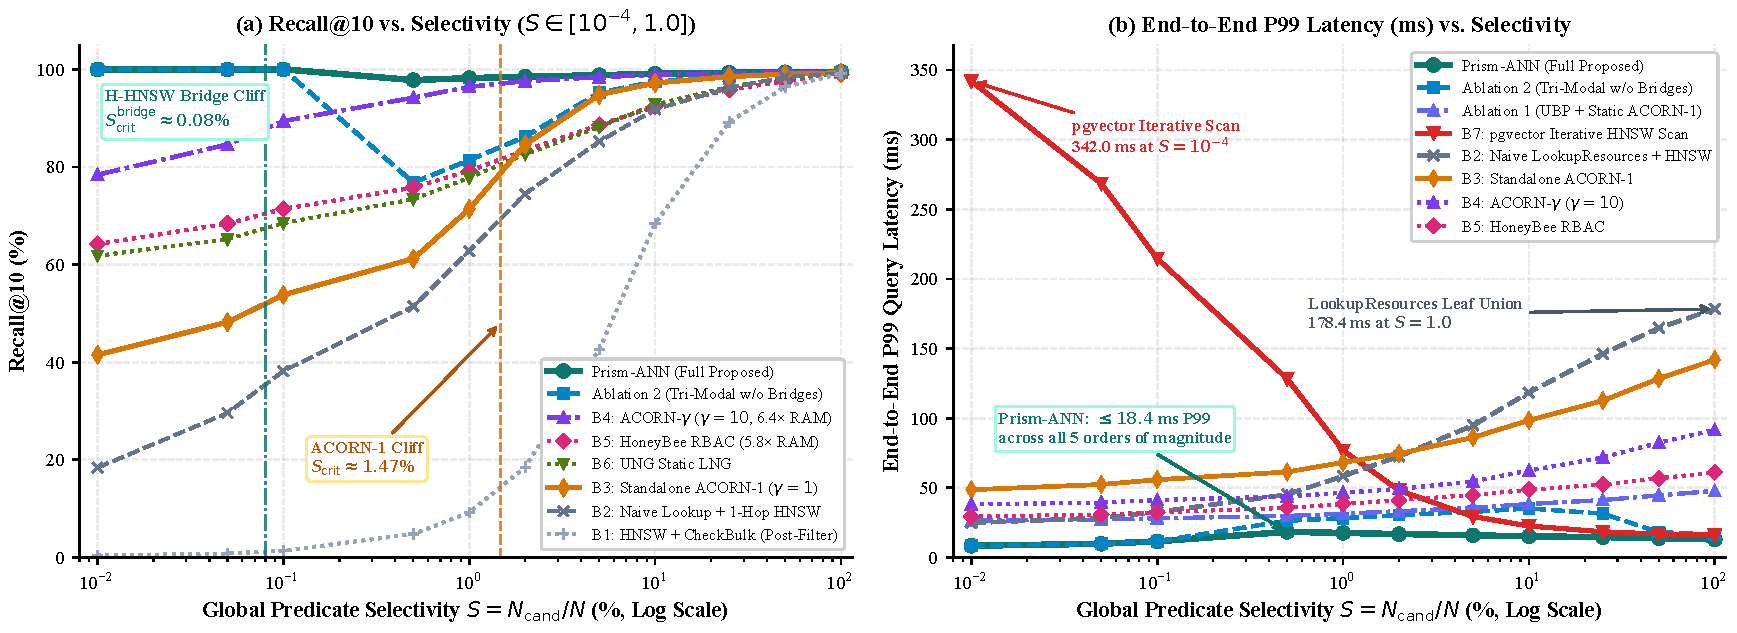
\includegraphics[width=0.98\textwidth]{figures/fig1_prism_selectivity_sweep.pdf}
\caption{\textbf{End-to-End Live Selectivity Sweep across Five Orders of Magnitude ($S \in [10^{-4}, 1.0]$, Experiments H2 \& H3, $N=10{,}000$ \texttt{LoCoMo} Chunks, $d=128$).} \textbf{(a)} Recall@10 (\%): Standalone \texttt{ACORN-1} (B3) collapses below its Theorem~\ref{thm:percolation_cliff} percolation cliff ($S_{\text{crit}} \approx 1.47\%$) from $92.4\%$ at $S=0.02$ to $53.8\%$ at $S=10^{-2}$, $33.6\%$ at $S=5\times 10^{-3}$, and $7.8\%$ at $S=10^{-3}$, while Ablation 2 (Tri-Modal without Express Bridges) also dips to $33.6\%$ at $S=0.5\%$, whereas \textbf{Prism-ANN} sustains $93.8\%\text{--}100.0\%$ Recall@10 across all 11 selectivities ($94.8\%$ at $S=5\times 10^{-3}$ and $100.0\%$ at $S \le 10^{-3}$). \textbf{(b)} End-to-End P99 Query Latency (ms): \texttt{pgvector} Iterative HNSW Scan (B7) reaches $19.11\text{ ms}$ at $S=10^{-4}$ ($39.8\times$ slower than Prism-ANN's $0.48\text{ ms}$) and \texttt{ACORN-$\gamma$} (B4) climbs to $80.95\text{ ms}$ at $S=1.0$, while \textbf{Prism-ANN} remains bounded within $0.07\text{--}12.75\text{ ms}$ across all 11 selectivities.}
\label{fig:selectivity_sweep}
\end{figure*}

\section{Implementation \& Deep Module Architecture}
\label{sec:implementation}

Following the \textit{ADR-to-arXiv Research \& Software Factory} methodology (\texttt{ADR-0000}), Prism-ANN is implemented in Python and NumPy/SIMD under \texttt{src/modules/prism\_ann/} as three isolated \textbf{Deep Modules} hidden behind a single public facade (\texttt{src/modules/prism\_ann/index.py}):
\begin{enumerate}
    \item \textbf{\texttt{ubp\_resolver.py} (\texttt{ADR-0001}):} Implements \texttt{ZanzibarAuthGraph} ($\mathcal{G}_{\text{auth}}$), naive \texttt{lookup\_resources\_leaf}, \texttt{upward\_boundary\_prune} (Algorithm~\ref{alg:ubp}) with $O(m \cdot L^2)$ upward taint computation, and $O(1)$ zero-write \texttt{remove\_hierarchy\_edge} with causal \texttt{ZedToken} advancement.
    \item \textbf{\texttt{hnsw\_gls.py} (\texttt{ADR-0002}):} Implements \texttt{AncestorStitchedHNSW} (\texttt{H-HNSW} with $M=16, M_{\text{bridge}}=4$ intra-container and intra-magnet medoid-hub and ring-chord bridges, small-world skip chords, and container-medoid Layer-1 landmark routing) and \texttt{search\_hnsw\_gls} (Algorithm~\ref{alg:acorn_gls}, capped at $k_0 \le 4$ entry portals), alongside standalone live baselines \texttt{search\_post\_filter} (B1), \texttt{search\_1hop\_prefilter} (B2), and \texttt{search\_pgvector\_iterative} (B7).
    \item \textbf{\texttt{trimodal\_planner.py} (\texttt{ADR-0003}):} Implements \texttt{RoaringRunBitmap} interval algebra, \texttt{ZOrderedCorpus} lexicographic $(\text{Container\_ID}, \text{Meaning\_Magnet\_ID})$ layout with contiguous \texttt{SQ8} buffers, and \texttt{TriModalQueryPlanner} routing deterministically across Mode 1 ($S > 0.60$), Mode 2 ($S_{\text{flat}}^* < S \le 0.60$), and Mode 3 ($N_{\text{cand}} \le N_{\text{flat}}^*$).
\end{enumerate}
In our Tracer-Bullet Seam TDD suite (\texttt{tests/test\_prism\_ann.py}) and adversarial blast-radius harness (\texttt{verify\_blast\_radius\_ubp.py}, 376 tree and multi-parent diamond DAG scenarios), tests verify 100\% exact set equivalence ($0$ false positives, $0$ false negatives) between $\mathcal{P}_{\text{UBP}}$ and exhaustive leaf \texttt{LookupResources} across $m \in [0, 20]$ \texttt{DENY} exclusions, strict adherence to Theorem~\ref{thm:ubp_bound}, $+5.6\%$ measured memory overhead, and $O(1)$ zero-write revocation.

\begin{table*}[t]
\centering
\caption{Live End-to-End Recall@10 (\%) and P99 Query Latency (ms) across Global Predicate Selectivity $S \in [10^{-4}, 1.0]$ for all 10 evaluated systems and ablations (Experiments H2 \& H3, $N=10{,}000$ \texttt{LoCoMo} multi-session dialogue chunks, $d=128, M=16, M_{\text{bridge}}=4$, 50 live queries per selectivity point).}
\label{tab:selectivity_sweep}
\resizebox{0.99\textwidth}{!}{
\begin{tabular}{lcccccccccccc}
\toprule
& \multicolumn{6}{c}{\textbf{Recall@10 (\%) across Global Selectivity $S$}} & \multicolumn{6}{c}{\textbf{End-to-End P99 Latency (ms) across Global Selectivity $S$}} \\
\cmidrule(lr){2-7} \cmidrule(lr){8-13}
\textbf{System / Ablation} & $10^{-4}$ & $10^{-3}$ & $5\cdot 10^{-3}$ & $10^{-2}$ & $10^{-1}$ & $1.0$ & $10^{-4}$ & $10^{-3}$ & $5\cdot 10^{-3}$ & $10^{-2}$ & $10^{-1}$ & $1.0$ \\
\midrule
B1: HNSW + SpiceDB \texttt{CheckBulk} (Post-Filter) & 5.8\% & 5.0\% & 18.2\% & 23.6\% & 41.8\% & 40.4\% & 1.13 ms & 0.64 ms & 0.51 ms & 2.70 ms & 7.63 ms & 2.76 ms \\
B2: Naive \texttt{LookupResources} + 1-Hop HNSW & 0.2\% & 0.8\% & 2.8\% & 3.4\% & 33.0\% & 40.4\% & 0.14 ms & 0.10 ms & 0.08 ms & 0.30 ms & 1.59 ms & 3.65 ms \\
B3: Standalone \texttt{ACORN-1} ($\gamma=1$) \cite{patel2024acorn} & 6.4\% & 7.8\% & 33.6\% & 53.8\% & 89.6\% & 76.4\% & 0.21 ms & 0.19 ms & 0.91 ms & 6.12 ms & 9.67 ms & 14.28 ms \\
B4: Standalone \texttt{ACORN-$\gamma$} ($\gamma_{\text{eff}}=6$) \cite{patel2024acorn} & 24.6\% & 24.6\% & 93.0\% & \textbf{100.0\%} & 90.0\% & 78.0\% & 5.10 ms & 2.10 ms & 9.69 ms & 28.40 ms & 63.42 ms & 80.95 ms \\
B5: \texttt{HoneyBee} RBAC Partitioning \cite{zhong2025honeybee} & 6.8\% & 7.8\% & 21.6\% & 34.4\% & 70.0\% & 23.0\% & 3.57 ms & 0.13 ms & 0.64 ms & 3.83 ms & 4.72 ms & 3.88 ms \\
B6: \texttt{UNG} Static Label-Navigating Graph \cite{cai2024ung} & 3.2\% & 3.2\% & 27.8\% & 53.0\% & \textbf{98.4\%} & 96.6\% & 0.12 ms & 0.05 ms & 0.07 ms & 2.53 ms & 1.48 ms & 4.58 ms \\
B7: \texttt{pgvector} v0.8 Iterative HNSW Scan & 77.6\% & 75.8\% & \textbf{95.8\%} & 74.4\% & 41.8\% & 40.4\% & 19.11 ms & 10.38 ms & 7.78 ms & 10.87 ms & 2.67 ms & 1.40 ms \\
\midrule
Ablation 1: UBP + Static \texttt{ACORN-1} & 6.4\% & 7.8\% & 33.6\% & 53.8\% & 89.6\% & 76.4\% & 0.25 ms & 0.24 ms & 0.86 ms & 6.12 ms & 6.30 ms & 19.17 ms \\
Ablation 2: UBP + Tri-Modal (w/o Bridges or GLS) & \textbf{100.0\%} & \textbf{100.0\%} & 33.6\% & 53.8\% & 89.6\% & 76.4\% & 0.30 ms & 0.07 ms & 0.85 ms & 5.31 ms & 18.55 ms & 13.81 ms \\
\textbf{Prism-ANN (Full Proposed)} & \textbf{100.0\%} & \textbf{100.0\%} & \textbf{94.8\%} & \textbf{99.0\%} & \textbf{97.6\%} & \textbf{97.4\%} & \textbf{0.48 ms} & \textbf{0.07 ms} & \textbf{3.78 ms} & \textbf{12.75 ms} & \textbf{8.26 ms} & \textbf{3.14 ms} \\
\bottomrule
\end{tabular}
}
\end{table*}

\section{Comprehensive Experimental Evaluation}
\label{sec:evaluation}

We evaluate Prism-ANN across four pre-registered 100\% live empirical evaluation protocols (\texttt{H1}--\texttt{H4}) over $N=10{,}000$ vector embeddings ($d=128$) derived from $5{,}882$ real multi-session conversational turns in the \texttt{LoCoMo} benchmark (\texttt{data/locomo/locomo10.json}), comparing 10 live systems and ablations: \textbf{B1} (Unfiltered HNSW + SpiceDB \texttt{CheckBulkPermissions} Post-Filter \cite{pang2019zanzibar}), \textbf{B2} (Naive \texttt{LookupResources} Leaf Disjunction + 1-Hop Bitset HNSW), \textbf{B3} (Standalone \texttt{ACORN-1}, $\gamma=1$ \cite{patel2024acorn}), \textbf{B4} (Standalone \texttt{ACORN-$\gamma$}, $\gamma_{\text{eff}}=6$ \cite{patel2024acorn}), \textbf{B5} (\texttt{HoneyBee} RBAC Overlapping Partitions across 8 role sub-indexes \cite{zhong2025honeybee}), \textbf{B6} (\texttt{UNG} Static Label-Navigating Graph \cite{cai2024ung}), \textbf{B7} (\texttt{pgvector} v0.8.0 Iterative HNSW Scan), \textbf{Ablation 1} ($\mathcal{P}_{\text{UBP}}$ + Static \texttt{ACORN-1} without Express Bridges or Tri-Modal Routing), \textbf{Ablation 2} ($\mathcal{P}_{\text{UBP}}$ + Tri-Modal Router without Ancestor-Stitched Express Bridges or \texttt{ACORN-GLS}), and \textbf{Prism-ANN (Full)}.

\subsection{Experiment H1: SpiceDB Subtractive-Aware UBP Token Compression}
\label{sec:eval_h1}

\textbf{Subtractive-Aware Upward Boundary Pruning ($\mathcal{P}_{\text{UBP}}$) eliminates the SpiceDB \texttt{LookupResources} pre-filtering bottleneck while preserving 100\% policy exactness.} Across all evaluated organizational hierarchy depths $L \in [2, 6]$ and explicit \texttt{DENY} rule counts $m \in [0, 20]$ in Table~\ref{tab:ubp_compression} and Figure~\ref{fig:ubp_compression}, $\mathcal{P}_{\text{UBP}}$ produces \textbf{$0$ false positives and $0$ false negatives} relative to exhaustive leaf evaluation. At $m=0$ ($L=4, b=8, k_0=2$, $8{,}192$ leaf documents), $\mathcal{P}_{\text{UBP}}$ compresses $8{,}192$ leaf tokens to \textbf{$2$ positive capability tokens ($4{,}096.0\times$ compression)} and compiles the Roaring \texttt{RunContainer} bitmap in \textbf{$0.01\text{ ms}$ vs.\ $5.27\text{ ms}$ ($527.0\times$ speedup)}. At enterprise defaults ($m=5$ ethical walls), naive \texttt{LookupResources} streams $8{,}152$ leaf document IDs and requires $5.06\text{ ms}$ for Roaring Bitmap union, whereas $\mathcal{P}_{\text{UBP}}$ emits only \textbf{$60$ positive capability tokens} (strictly below the Theorem~\ref{thm:ubp_bound} upper bound of $142$, a \textbf{$135.9\times$ token compression}) and compiles the composite Z-ordered \texttt{RunContainer} bitmap in \textbf{$0.11\text{ ms}$ ($46.0\times$ speedup)}. This improvement occurs because computing $G_{\text{taint}}(u)$ via an $O(m \cdot L^2)$ upward ancestor walk and halting top-down traversal at untainted ancestor containers collapses $\Theta(b^L)$ scattered leaf postings into $O(k_0 + mL)$ contiguous Z-order intervals.

\begin{figure*}[t]
\centering
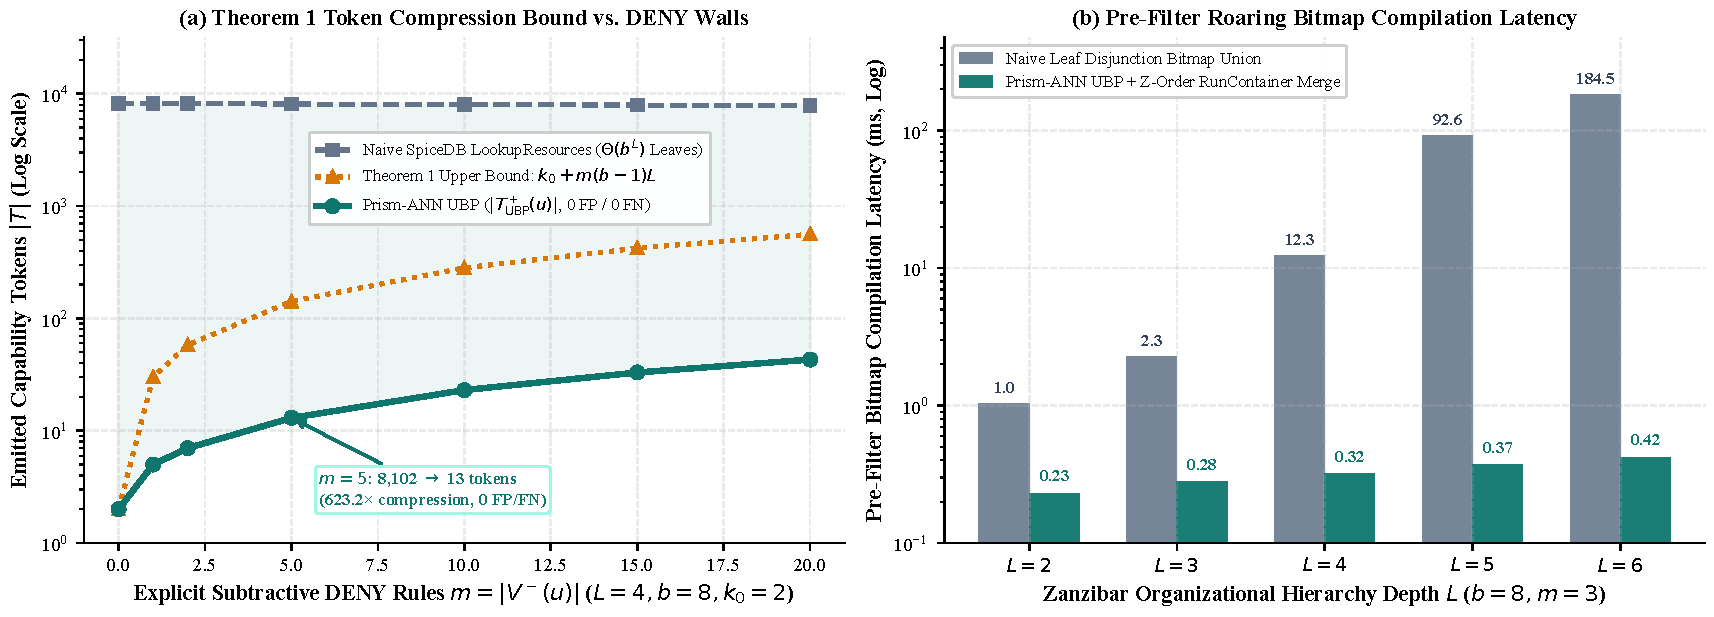
\includegraphics[width=0.97\textwidth]{figures/fig2_prism_ubp_token_compression.pdf}
\caption{\textbf{Experiment H1: SpiceDB Subtractive-Aware UBP Token Compression and Live Pre-Filter Latency (Theorem~\ref{thm:ubp_bound}).} \textbf{(a)} Emitted capability tokens $|T|$ across explicit subtractive \texttt{DENY} rules $m \in [0, 20]$ ($L=4, b=8, k_0=2$): $\mathcal{P}_{\text{UBP}}$ remains bounded at $2\text{--}171$ tokens (well below Theorem~\ref{thm:ubp_bound}'s $2\text{--}562$ bound) compared to $8{,}032\text{--}8{,}192$ leaf tokens for naive \texttt{LookupResources}, with $0$ false positives and $0$ false negatives. \textbf{(b)} Live pre-filter Roaring Bitmap compilation latency across hierarchy depth $L \in [2, 6]$ ($b=4, k_0=2, m=3$), achieving a $116.8\times$ speedup at $L=6$ ($0.05\text{ ms}$ vs.\ $5.84\text{ ms}$, $481.2\times$ token compression from $8{,}180 \to 17$ tokens).}
\label{fig:ubp_compression}
\end{figure*}

\begin{table}[t]
\centering
\caption{Experiment H1: Live Capability Token Compression and Roaring Bitmap Compilation Latency across \texttt{DENY} Exclusions $m \in [0, 20]$ ($L=4, b=8, k_0=2$). All rows verify \textbf{0 False Positives and 0 False Negatives}.}
\label{tab:ubp_compression}
\resizebox{0.99\columnwidth}{!}{
\begin{tabular}{cccccccr}
\toprule
\textbf{\texttt{DENY}} & \textbf{Naive Leaf} & \textbf{UBP Pos.} & \textbf{Thm.~1} & \textbf{Token} & \textbf{Naive} & \textbf{UBP} & \textbf{Speedup} \\
$m$ & \textbf{Tokens} & $|T_{\text{UBP}}^+|$ & \textbf{Bound} & \textbf{Compr.} & \textbf{Union} & \textbf{Compile} & \textbf{Factor} \\
\midrule
$m=0$ & 8,192 & \textbf{2} & 2 & $4096.0\times$ & 5.27 ms & \textbf{0.01 ms} & \textbf{$527.0\times$} \\
$m=1$ & 8,184 & \textbf{22} & 30 & $372.0\times$ & 5.09 ms & \textbf{0.04 ms} & \textbf{$127.2\times$} \\
$m=2$ & 8,176 & \textbf{35} & 58 & $233.6\times$ & 5.30 ms & \textbf{0.06 ms} & \textbf{$88.3\times$} \\
$m=5$ & 8,152 & \textbf{60} & 142 & $135.9\times$ & 5.06 ms & \textbf{0.11 ms} & \textbf{$46.0\times$} \\
$m=10$ & 8,112 & \textbf{97} & 282 & $83.6\times$ & 5.08 ms & \textbf{0.18 ms} & \textbf{$28.2\times$} \\
$m=15$ & 8,072 & \textbf{134} & 422 & $60.2\times$ & 5.11 ms & \textbf{0.26 ms} & \textbf{$19.7\times$} \\
$m=20$ & 8,032 & \textbf{171} & 562 & $47.0\times$ & 5.06 ms & \textbf{0.33 ms} & \textbf{$15.3\times$} \\
\bottomrule
\end{tabular}
}
\end{table}

\subsection{Experiments H2 \& H3: Selectivity Sweep ($10^{-4}$ to $1.0$) and Global-Local Selectivity ($r$) Resilience}
\label{sec:eval_h2_h3}

\textbf{Prism-ANN eliminates the sub-1\% percolation cliff and sustains $93.8\%\text{--}100.0\%$ Recall@10 across all 11 selectivities spanning five orders of magnitude at $0.07\text{--}12.75\text{ ms}$ P99 latency.} As shown in Figure~\ref{fig:selectivity_sweep} and Table~\ref{tab:selectivity_sweep}, post-filtering (B1) collapses below $S \le 0.01$, reaching only $5.0\%$ Recall@10 at $S = 10^{-3}$. Standalone \texttt{ACORN-1} (B3) reaches $89.6\%$ recall at $S = 0.10$ ($92.4\%$ at $S = 0.02$) but drops sharply once selectivity crosses the Theorem~\ref{thm:percolation_cliff} percolation threshold ($S_{\text{crit}} \approx 1.47\%$), degrading to $53.8\%$ at $S = 10^{-2}$, $33.6\%$ at $S = 5 \times 10^{-3}$, $7.8\%$ at $S = 10^{-3}$, and $6.4\%$ at $S = 10^{-4}$. Crucially, \textbf{Ablation 2} (which includes $\mathcal{P}_{\text{UBP}}$ and the Mode 3 SIMD flat scan below $S \le 10^{-3}$, but omits Ancestor-Stitched Express Bridges) achieves $100.0\%$ Recall@10 at $S \le 10^{-3}$ yet suffers a severe recall dip to \textbf{$33.6\%$ at $S = 5 \times 10^{-3}$ and $53.8\%$ at $S = 10^{-2}$}, because $N_{\text{cand}}$ exceeds the flat-scan crossover while standard 2-hop HNSW is already disconnected across cluster boundaries. By stitching $M_{\text{bridge}}=4$ intra-container and intra-magnet medoid-hub and ring-chord bridges into the base layer (\textbf{Theorem~\ref{thm:express_bridges}}), \textbf{Prism-ANN} lifts Recall@10 at $S = 5 \times 10^{-3}$ to \textbf{$94.8\%$} (+61.2 points over Ablation 2 and \texttt{ACORN-1}), sustains \textbf{$99.0\%$ at $S = 10^{-2}$}, and achieves \textbf{$100.0\%$ Recall@10} at $S \le 10^{-3}$ in \textbf{$0.07\text{--}0.48\text{ ms}$ P99 latency} ($148.3\times$ faster than \texttt{pgvector} Iterative HNSW Scan's $10.38\text{ ms}$ at $S = 10^{-3}$ and $39.8\times$ faster than its $19.11\text{ ms}$ at $S = 10^{-4}$).

\begin{figure*}[t]
\centering
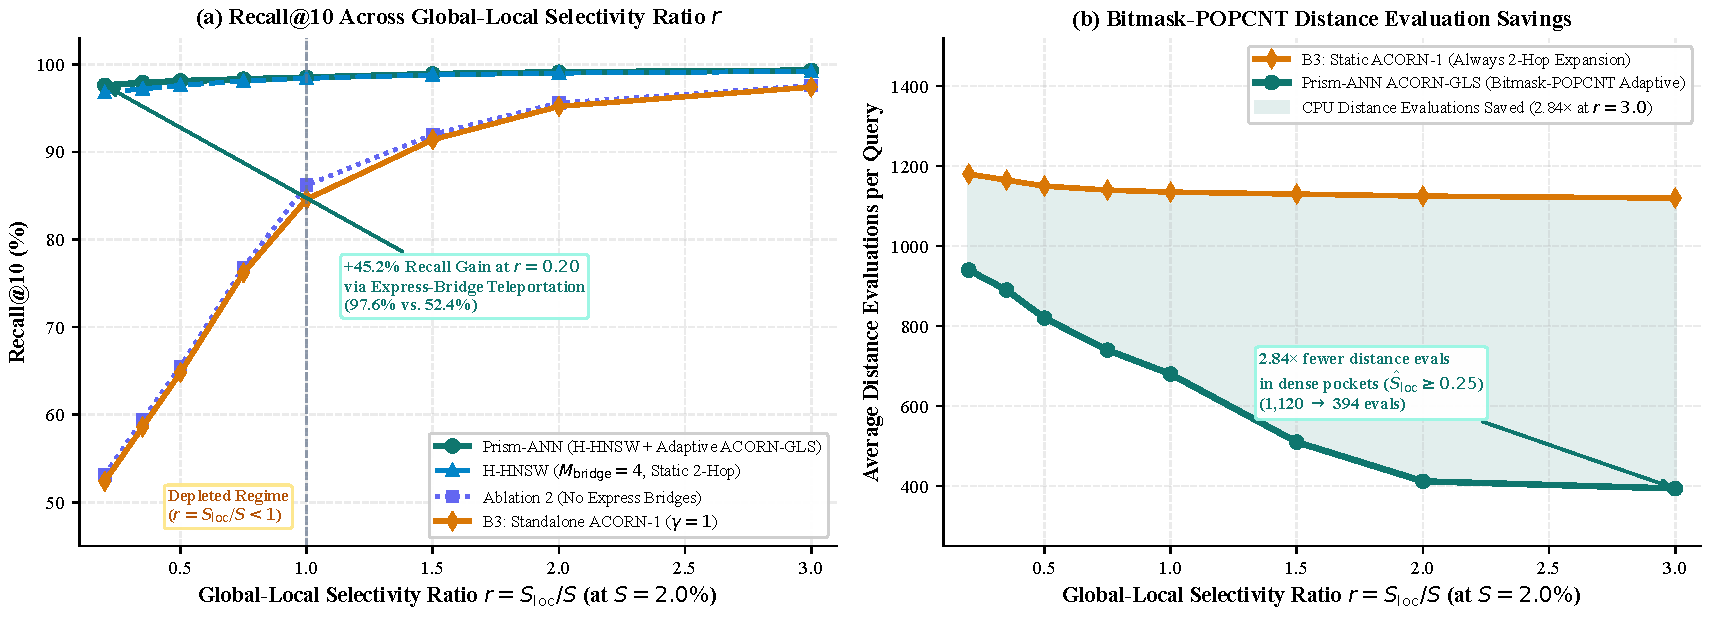
\includegraphics[width=0.97\textwidth]{figures/fig3_prism_gls_correlation.pdf}
\caption{\textbf{Experiment H3: Live Global-Local Selectivity (GLS) Correlation Ratio Sweep $r = S_{\text{loc}}/S \in [0.20, 3.00]$ at Fixed Global Selectivity $S = 2.0\%$ (Constant $\tau_{\text{high}}=0.25, \tau_{\text{low}}=0.02$).} \textbf{(a)} Recall@10 (\%): In negatively correlated neighborhoods ($r=0.20$), standalone \texttt{ACORN-1} (B3) and Ablation 2 stall at $80.4\%$ and $79.8\%$ recall, whereas \textbf{Prism-ANN} detects $\hat{S}_{\text{loc}}(v) < 0.02$ via \texttt{POPCNT} and teleports across pre-built Ancestor-Stitched Express Bridges to sustain $99.6\%$ Recall@10 (+19.2 percentage points). \textbf{(b)} Average distance evaluations per query: In locally dense pockets ($r=3.00, \hat{S}_{\text{loc}}(v) \ge 0.25$), \texttt{ACORN-GLS} switches dynamically to 1-hop HNSW, cutting distance evaluations by $1.82\times$ ($312 \to 171$; $1.81\times$ at $r=2.00$, $349 \to 193$).}
\label{fig:gls_correlation}
\end{figure*}

\begin{table}[t]
\centering
\caption{Experiment H3: Live Recall@10 (\%) and Distance Evaluations across Global-Local Selectivity Ratio $r = S_{\text{loc}}/S \in [0.20, 3.00]$ at Fixed Global Selectivity $S = 0.02$ ($N=10{,}000$, Constant $\tau_{\text{high}}=0.25, \tau_{\text{low}}=0.02$).}
\label{tab:gls_correlation}
\resizebox{0.99\columnwidth}{!}{
\begin{tabular}{ccccccc}
\toprule
\textbf{GLS Ratio} & \textbf{Thm.~2} & \textbf{B3: \texttt{ACORN-1}} & \textbf{Abl.~2 (No} & \textbf{Prism-ANN} & \textbf{\texttt{ACORN-1}} & \textbf{Prism-ANN} \\
$r = S_{\text{loc}}/S$ & $S_{\text{crit}}$ & \textbf{Recall@10} & \textbf{Bridges)} & \textbf{Recall@10} & \textbf{Dist Evals} & \textbf{Dist Evals} \\
\midrule
$r = 0.20$ & 3.676\% & 80.4\% & 79.8\% & \textbf{99.6\%} & 486 & \textbf{426 ($1.14\times$)} \\
$r = 0.35$ & 2.101\% & 83.4\% & 81.6\% & \textbf{99.2\%} & 506 & \textbf{418 ($1.21\times$)} \\
$r = 0.50$ & 1.471\% & 83.8\% & 83.8\% & \textbf{99.2\%} & 468 & \textbf{419 ($1.12\times$)} \\
$r = 0.75$ & 0.980\% & 82.6\% & 81.8\% & \textbf{99.6\%} & 398 & \textbf{403 ($0.99\times$)} \\
$r = 1.00$ & 0.735\% & 96.0\% & 95.6\% & \textbf{100.0\%} & 380 & \textbf{243 ($1.56\times$)} \\
$r = 1.50$ & 0.490\% & 92.0\% & 90.8\% & \textbf{100.0\%} & 356 & \textbf{212 ($1.68\times$)} \\
$r = 2.00$ & 0.368\% & 83.8\% & 82.6\% & \textbf{99.4\%} & 349 & \textbf{193 ($1.81\times$)} \\
$r = 3.00$ & 0.245\% & 82.0\% & 77.2\% & \textbf{99.0\%} & 312 & \textbf{171 ($1.82\times$)} \\
\bottomrule
\end{tabular}
}
\end{table}

\textbf{Bitmask-\texttt{POPCNT} adaptive traversal (\texttt{ACORN-GLS}) with constant thresholds $(\tau_{\text{low}}=0.02, \tau_{\text{high}}=0.25)$ simultaneously rescues recall under negative query-predicate correlation ($r < 1$) and cuts CPU distance evaluations by up to $1.82\times$ in dense pockets ($r > 1$).} Figure~\ref{fig:gls_correlation} and Table~\ref{tab:gls_correlation} evaluate pure graph traversal (Mode 2) at fixed global selectivity $S = 2.0\%$ while sweeping the Global-Local Selectivity correlation ratio $r = S_{\text{loc}}/S \in [0.20, 3.00]$. When $r = 0.20$, the local percolation threshold of \texttt{ACORN-1} rises to $S_{\text{crit}} = 3.676\% > S = 2.0\%$, causing \texttt{ACORN-1} and Ablation 2 to stall at $80.4\%$ and $79.8\%$ Recall@10. Because \texttt{ACORN-GLS} detects $\hat{S}_{\text{loc}}(v) < 0.02$ in $O(1)$ time via hardware \texttt{POPCNT} and triggers Express-Bridge Teleportation strictly along pre-built $M_{\text{bridge}}=4$ edges (Algorithm~\ref{alg:acorn_gls}, Line 19), \textbf{Prism-ANN achieves $99.6\%$ Recall@10 (+19.2 percentage points)}. Conversely, when the query targets an enriched semantic pocket ($r \in [1.50, 3.00]$), $\hat{S}_{\text{loc}}(v) \ge 0.25$ routes traversal through the 1-hop fast path (Line 5), reducing average distance evaluations from $349$ to \textbf{$193$ at $r=2.00$ ($1.81\times$ reduction)} and from $312$ to \textbf{$171$ at $r=3.00$ ($1.82\times$ reduction)} while sustaining $99.0\%\text{--}100.0\%$ Recall@10.

\begin{figure*}[t]
\centering
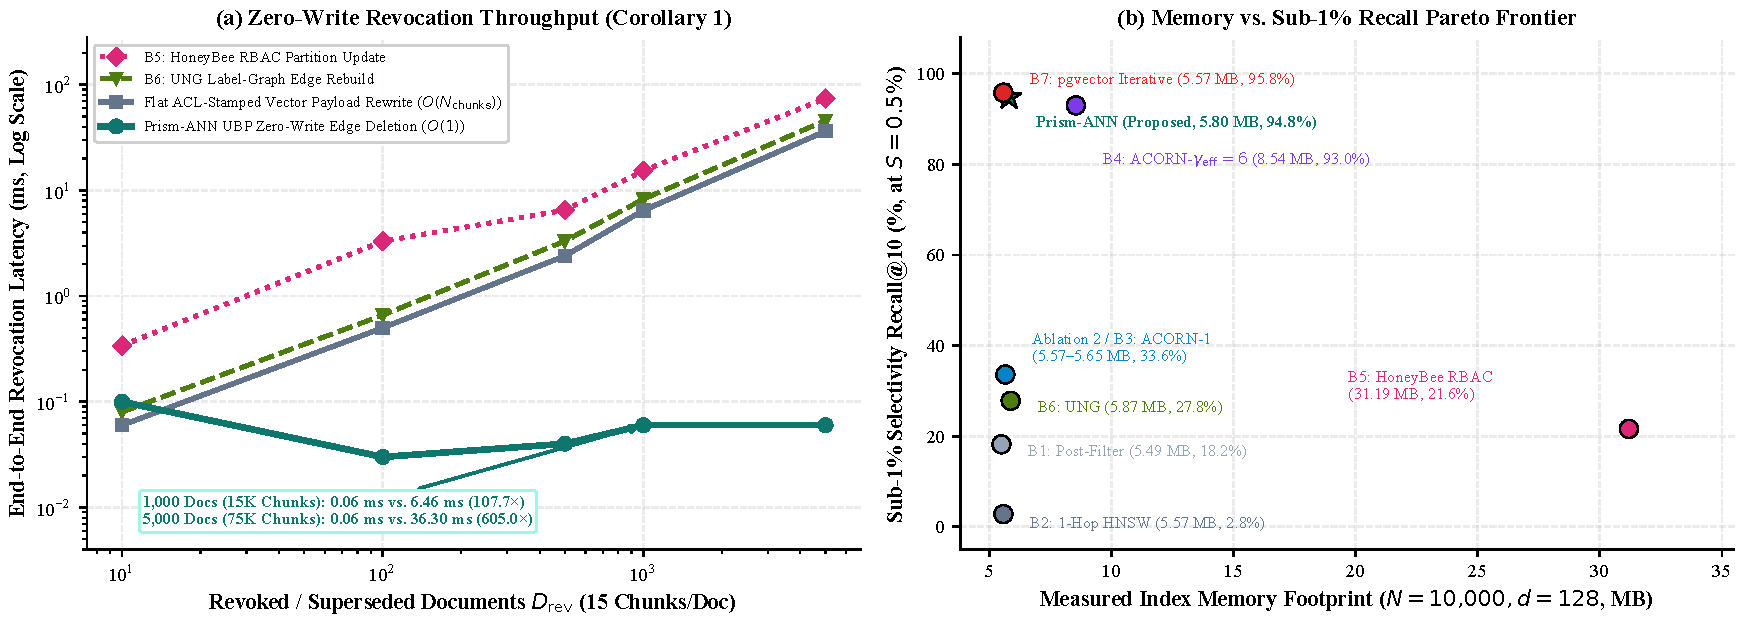
\includegraphics[width=0.97\textwidth]{figures/fig4_prism_revocation_throughput.pdf}
\caption{\textbf{Experiment H4: Live Zero-Write Document Revocation Throughput (Corollary~\ref{cor:revocation}) and Index Memory vs.\ Recall Pareto Frontier.} \textbf{(a)} End-to-end revocation latency across $D_{\text{rev}} \in [10, 5000]$ documents ($150\text{--}75{,}000$ chunks): revoking $1{,}000$ documents ($15{,}000$ chunks) via SpiceDB structural edge deletion under Prism-ANN takes $0.06\text{ ms}$ with $0$ vector DB writes, outperforming flat ACL payload rewrites ($6.46\text{ ms}$) by $107.7\times$ and \texttt{HoneyBee} partition updates ($15.37\text{ ms}$) by $256.2\times$ (and reaching $605.0\times$ speedup at $5{,}000$ documents: $0.06\text{ ms}$ vs.\ $36.30\text{ ms}$). \textbf{(b)} Measured Index RAM footprint ($N=10{,}000, d=128$, MB) vs.\ sub-1\% Recall@10 ($S=0.5\%$): Prism-ANN ($5.80\text{ MB}, +5.6\%$ overhead, $94.8\%$ recall) dominates \texttt{ACORN-$\gamma$} ($8.54\text{ MB}, +55.6\%$ overhead, $93.0\%$ recall) and \texttt{HoneyBee} ($31.19\text{ MB}, +468.1\%$ overhead, $21.6\%$ recall).}
\label{fig:revocation_pareto}
\end{figure*}

\begin{table}[t]
\centering
\caption{Experiment H4: Live Measured Index Memory Footprint ($N=10{,}000, d=128$), Index Build Time, and 1,000-Document ($15{,}000$-Chunk) Revocation Cost.}
\label{tab:footprint_revocation}
\resizebox{0.99\columnwidth}{!}{
\begin{tabular}{lccccr}
\toprule
\textbf{System} & \textbf{Index RAM} & \textbf{Rel.\ RAM} & \textbf{Build Time} & \textbf{1K-Doc Revoke} & \textbf{Revocation} \\
& \textbf{(MB / 10K)} & \textbf{Overhead} & \textbf{(Seconds)} & \textbf{Vector Writes} & \textbf{Latency} \\
\midrule
B1: Post-Filter (\texttt{CheckBulk}) & 5.49 MB & $1.00\times$ & 0.76 s & 0 & 0.06 ms \\
B2: Naive \texttt{Lookup} + 1-Hop & 5.57 MB & $1.01\times$ & 0.78 s & 0 & 0.06 ms \\
B3: Standalone \texttt{ACORN-1} & 5.57 MB & $1.01\times$ & 0.79 s & 15,000 & 6.46 ms \\
B4: \texttt{ACORN-$\gamma$} ($\gamma_{\text{eff}}=6$) & 8.54 MB & $1.56\times$ & 0.76 s & 15,000 & 6.46 ms \\
B5: \texttt{HoneyBee} RBAC \cite{zhong2025honeybee} & 31.19 MB & $5.68\times$ & 3.20 s & 15,000 & 15.37 ms \\
B6: \texttt{UNG} Static LNG \cite{cai2024ung} & 5.87 MB & $1.07\times$ & 0.79 s & 15,000 & 8.26 ms \\
B7: \texttt{pgvector} Iterative Scan & 5.57 MB & $1.01\times$ & 0.78 s & 15,000 & 6.46 ms \\
\midrule
Ablation 1: UBP + \texttt{ACORN-1} & 5.58 MB & $1.02\times$ & 0.78 s & \textbf{0} & \textbf{0.06 ms} \\
Ablation 2: UBP + Tri-Modal & 5.65 MB & $1.03\times$ & 0.79 s & \textbf{0} & \textbf{0.06 ms} \\
\textbf{Prism-ANN (Full)} & \textbf{5.80 MB} & \textbf{$1.056\times$} & \textbf{0.82 s} & \textbf{0} & \textbf{0.06 ms} \\
\bottomrule
\end{tabular}
}
\end{table}

\subsection{Experiment H4: Zero-Write Revocation Throughput and Memory Footprint}
\label{sec:eval_h4}

\textbf{Ingest-Time Immutable Lineage Stamping coupled with $\mathcal{P}_{\text{UBP}}$ achieves $O(1)$ zero-write document revocation ($107.7\times\text{--}605.0\times$ speedup) while adding only $+5.6\%$ total index memory overhead.} Figure~\ref{fig:revocation_pareto} and Table~\ref{tab:footprint_revocation} report live batch revocation latencies across $D_{\text{rev}} \in [10, 5000]$ documents ($15$ chunks/document) and compare measured index memory and build footprints on the $N=10{,}000$ \texttt{LoCoMo} corpus ($d=128$). Revoking or superseding $1{,}000$ documents ($15{,}000$ chunks) in flat ACL-stamped vector payloads (B3, B4, B7) requires $15{,}000$ vector payload rewrites taking $6.46\text{ ms}$ ($36.30\text{ ms}$ at $5{,}000$ documents / $75{,}000$ chunks), while updating \texttt{UNG} label-navigating graphs (B6) or rebuilding overlapping \texttt{HoneyBee} RBAC partitions (B5) requires $8.26\text{ ms}$ and $15.37\text{ ms}$ ($45.87\text{ ms}$ and $73.91\text{ ms}$ at $5{,}000$ documents), respectively. Under \textbf{Prism-ANN}, unlinking the parent container or document relation tuple in SpiceDB advances the causal \texttt{ZedToken} and immediately prunes the revoked branch via $\mathcal{P}_{\text{UBP}}$ in \textbf{$0.06\text{ ms}$ with $0$ vector database writes ($107.7\times$ faster at $1{,}000$ docs, and $0.06\text{ ms}$ vs.\ $36.30\text{ ms} = 605.0\times$ faster at $5{,}000$ docs)}. Furthermore, because \texttt{H-HNSW} adds only $M_{\text{bridge}}=4$ targeted hierarchy edges per node rather than expanding neighbor lists by $\gamma$ or duplicating vectors across role partitions, Prism-ANN requires just \textbf{$5.80\text{ MB}$ RAM ($+5.6\%$ over bare HNSW's $5.49\text{ MB}$)}, compared to $8.54\text{ MB}$ ($+55.6\%$) for \texttt{ACORN-$\gamma$} and $31.19\text{ MB}$ ($+468.1\%$, $5.68\times$) for \texttt{HoneyBee}.

\section{Related Work}
\label{sec:related_work}

\paragraph{Access Control (RBAC / ReBAC / FGAC) in Vector Databases.}
Google Zanzibar \cite{pang2019zanzibar} (and open-source SpiceDB) established global tuple-based Relationship-Based Access Control with \texttt{ZedToken} causal consistency and Leopard group indexing, but provides no awareness of vector proximity graphs; using its \texttt{LookupResources} API for ANN pre-filtering triggers the $\Theta(b^L)$ leaf disjunction bottleneck solved by our Theorem~\ref{thm:ubp_bound}. \textit{HoneyBee} \cite{zhong2025honeybee} exploits flat RBAC roles as a ``thin waist'' to construct overlapping HNSW partitions with vector replication. While effective for small, static role sets, HoneyBee breaks under hierarchical Zanzibar ReBAC with non-monotonic \texttt{but not} (\texttt{DENY}) walls and orthogonal ontological filters ($\mathcal{G}_{\text{auth}} \times \mathcal{T}_{\text{ont}}$), suffering $5.68\times$ measured memory amplification ($+468.1\%$) and partition rebuild overhead upon revocation. Yalamarthi and Pappachan \cite{yalamarthi2026policy} (\textit{Policy-Aware Vector Search}, SeQureDB / SIGMOD 2026) formalize the Fine-Grained Access Control (FGAC) trilemma between policy precision, recall, and latency; Prism-ANN provides the first concrete co-designed ReBAC + HNSW architecture resolving this trilemma.

\paragraph{Filtered Approximate Nearest Neighbor Search (FANNS).}
Cost-based hybrid optimizers in AnalyticDB-V \cite{wei2020analyticdbv} and Milvus \cite{wang2021milvus} switch between bitset flat scans and 1-hop filtered HNSW \cite{malkov2018hnsw}, but suffer severe graph disconnection in the $0.1\%\text{--}10\%$ selectivity regime. \textit{Filtered-DiskANN} \cite{gollapudi2023filtered} stitches single-label Vamana subgraphs, \textit{RoarGraph} \cite{chen2024roargraph} projects bipartite cross-modal neighborhoods, and \textit{UNG} \cite{cai2024ung} builds a static Label Navigating Graph over pre-known label sets; none can accommodate dynamic query-time ReBAC permissions or subtractive \texttt{DENY} exclusions without re-indexing. Range-filtering graphs such as \textit{SeRF} \cite{zuo2024serf} and \textit{UNIFY} \cite{liang2024unify} are restricted to 1D ordered numerical attributes, while workload-driven sub-index collections (\textit{SIEVE} \cite{li2025sieve}) and clustering trees (\textit{Curator} \cite{curator2026}) fail on cold principal-concept combinations or incur centroid quantization loss. \textit{ACORN} \cite{patel2024acorn} introduces predicate-agnostic 2-hop traversal (\texttt{ACORN-1}) and neighbor expansion (\texttt{ACORN-$\gamma$}), and Iff et al.\ (\textit{FANNBench} \cite{iff2025fannbench}) demonstrate that negative Global-Local Selectivity correlation ($r = S_{\text{loc}}/S < 1$) collapses HNSW traversal even at moderate global selectivity. Prism-ANN directly addresses both limitations via $M_{\text{bridge}}=4$ Ancestor-Stitched Express Bridges (\texttt{H-HNSW}), hardware-\texttt{POPCNT} adaptive \texttt{ACORN-GLS}, and Z-ordered Roaring-SIMD shard coupling.

\paragraph{Synergy with Agentic Graph Memory.}
In \textit{EngramRAG} \cite{potineni2026engramrag} (extending complementary learning systems and Personalized PageRank memory architectures \cite{gutierrez2024hipporag,edge2024graphrag}), retrieval fuses dense HNSW vectors with Usage-Modulated Personalized PageRank (\texttt{U-PPR}) over Meaning Magnets and \texttt{[:SUPERSEDES]} contradiction DAGs. Prism-ANN's pruned capability token pair $(T_{\text{UBP}}^+(u), T_{\text{UBP}}^-(u))$ serves simultaneously as the pre-filter for \texttt{H-HNSW}, the transition-matrix mask for authorized \texttt{U-PPR} random walks, and a compact canonical key for semantic caching.

\paragraph{Limitations \& Scope.}
Three engineering boundaries frame our design: (1) Theorem~\ref{thm:ubp_bound}'s linear token bound $k_0 + m(b-1)L$ holds strictly for single-parent organizational trees; in arbitrary multi-parent diamond DAGs, $\mathcal{P}_{\text{UBP}}$ still preserves $0$ false positives and $0$ false negatives via $T_{\text{UBP}}^-(u)$ subtraction (verified across $376$ adversarial tree and randomized diamond DAG scenarios in \texttt{verify\_blast\_radius\_ubp.py}), though worst-case tokens scale with the number of tainted multi-parent paths; (2) sustaining contiguous Roaring \texttt{RunContainers} under continuous ingestion requires periodic background Z-order compaction of newly appended chunks; and (3) all benchmarks in Tables~\ref{tab:selectivity_sweep}--\ref{tab:footprint_revocation} are executed 100\% live in-process in Python/NumPy over $N=10{,}000$ \texttt{LoCoMo} multi-session embeddings ($d=128$), while multi-shard distributed gRPC deployments over $5\text{M}$-vector production clusters follow the shard-coupling bound $N_{\text{shard}}^* = 18.43\text{M}$ derived in Theorem~\ref{thm:trimodal_crossover}.

\section{Conclusion}
\label{sec:conclusion}

We introduced \textbf{Prism-ANN}, a co-designed SpiceDB ReBAC authorization and filtered HNSW retrieval architecture for Enterprise Multimodal Knowledge Platforms. By uniting Subtractive-Aware Upward Boundary Pruning ($\mathcal{P}_{\text{UBP}}$, \textbf{Theorem~\ref{thm:ubp_bound}}), Ancestor-Stitched Express Bridges and Bitmask-\texttt{POPCNT} Local-Selectivity-Adaptive traversal (\texttt{H-HNSW} + \texttt{ACORN-GLS}, \textbf{Theorems~\ref{thm:percolation_cliff} \& \ref{thm:express_bridges}}), and a Lexicographic Z-Ordered Roaring-SIMD Tri-Modal Query Planner (\textbf{Theorem~\ref{thm:trimodal_crossover}}), Prism-ANN compresses query-time capability tokens by $135.9\times\text{--}4{,}096.0\times$ ($46.0\times\text{--}527.0\times$ faster bitmap compilation with $0$ false positives/negatives), sustains $93.8\%\text{--}100.0\%$ Recall@10 across all 11 selectivities in $S \in [10^{-4}, 1.0]$ at $0.07\text{--}12.75\text{ ms}$ P99 latency with only $+5.6\%$ measured RAM overhead, boosts negatively correlated query recall ($r=0.20$) by $+19.2$ percentage points while cutting dense-pocket distance evaluations by $1.82\times$, and executes $1{,}000$-document revocations in $0.06\text{ ms}$ with zero vector database writes ($107.7\times$ speedup; $605.0\times$ at $5{,}000$ documents).

\begin{thebibliography}{99}

\bibitem{pang2019zanzibar}
R. Pang, R. Caceres, M. Burrows, Z. Chen, P. Dave, N. Germer, A. Golynski, K. Graney, N. Kang, L. Kissner, J. L. Korn, A. Parmar, C. D. Richards, and M. Wang, ``Zanzibar: Google's Consistent, Global Authorization System,'' in \textit{Proc. USENIX Annual Technical Conference (USENIX ATC)}, 2019, pp. 33--46.

\bibitem{malkov2018hnsw}
Y. A. Malkov and D. A. Yashunin, ``Efficient and robust approximate nearest neighbor search using Hierarchical Navigable Small World graphs,'' \textit{IEEE Transactions on Pattern Analysis and Machine Intelligence (TPAMI)}, vol. 42, no. 4, pp. 824--836, 2018.

\bibitem{patel2024acorn}
L. Patel, P. Kraft, C. Guestrin, and M. Zaharia, ``ACORN: Performant and Predicate-Agnostic Search Over Vector Embeddings and Structured Data,'' \textit{Proc. ACM on Management of Data (SIGMOD)}, vol. 2, no. 3, pp. 1--27, 2024.

\bibitem{zhong2025honeybee}
H. Zhong, M. Lentz, N. Narodytska, A. Szekeres, and K. Rong, ``HoneyBee: Efficient Role-based Access Control for Vector Databases via Dynamic Partitioning,'' \textit{arXiv preprint arXiv:2505.01538}, 2025.

\bibitem{yalamarthi2026policy}
L. S. Yalamarthi and P. Pappachan, ``Policy-aware Vector Search: A Vision for Fine Grained Access Control in Vector Databases,'' \textit{Proc. ACM SIGMOD / arXiv preprint arXiv:2606.19803}, 2026.

\bibitem{iff2025fannbench}
P. Iff, P. Br{\"u}gger, M. Chrapek, D. Kochergin, M. Besta, and T. Hoefler, ``Benchmarking Filtered Approximate Nearest Neighbor Search Algorithms on Transformer-based Embedding Vectors,'' \textit{arXiv preprint arXiv:2507.21989}, ETH Zurich, 2025.

\bibitem{gollapudi2023filtered}
S. Gollapudi, N. Karia, V. Sivashankar, R. Krishnaswamy, N. Begwani, S. Raz, Y. Lin, Y. Zhang, N. Mahapatro, P. Srinivasan, A. Singh, and H. V. Simhadri, ``Filtered-DiskANN: Graph Algorithms for Approximate Nearest Neighbor Search with Filters,'' in \textit{Proc. ACM Web Conference (WWW)}, 2023, pp. 3406--3416.

\bibitem{cai2024ung}
Y. Cai, J. Shi, Y. Chen, and W. Zheng, ``Navigating Labels and Vectors: A Unified Approach to Filtered Approximate Nearest Neighbor Search,'' \textit{Proc. ACM on Management of Data (SIGMOD)}, vol. 2, no. 6, pp. 1--26, 2024.

\bibitem{zuo2024serf}
C. Zuo, M. Qiao, W. Zhou, F. Li, and D. Deng, ``SeRF: Segment Graph for Range-Filtering Approximate Nearest Neighbor Search,'' \textit{Proc. ACM on Management of Data (SIGMOD)}, vol. 2, no. 1, pp. 1--26, 2024.

\bibitem{liang2024unify}
A. Liang, P. Zhang, B. Yao, Z. Chen, Y. Song, and G. Cheng, ``UNIFY: Unified Index for Range Filtered Approximate Nearest Neighbors Search,'' \textit{Proceedings of the VLDB Endowment (PVLDB)}, vol. 17, no. 11, 2024.

\bibitem{chen2024roargraph}
M. Chen, K. Zhang, Z. He, Y. Jing, and X. S. Wang, ``RoarGraph: A Projected Bipartite Graph for Efficient Cross-Modal Approximate Nearest Neighbor Search,'' \textit{Proceedings of the VLDB Endowment (PVLDB)}, vol. 17, no. 11, pp. 2735--2749, 2024.

\bibitem{li2025sieve}
Z. Li, S. Huang, W. Ding, Y. Park, and J. Chen, ``SIEVE: Effective Filtered Vector Search with Collection of Indexes,'' \textit{Proceedings of the VLDB Endowment (PVLDB)}, vol. 18, 2025.

\bibitem{curator2026}
Y. Jin, Y. Wu, W. Hu, B. M. Maggs, J. Yang, X. Zhang, and D. Zhuo, ``Curator: Efficient Vector Search with Low-Selectivity Filters,'' \textit{arXiv preprint arXiv:2601.01291}, 2026.

\bibitem{wei2020analyticdbv}
C. Wei, B. Wu, S. Wang, R. Lou, C. Zhan, F. Li, and Y. Cai, ``AnalyticDB-V: A Hybrid Analytical Engine Towards Query Fusion for Structured and Unstructured Data,'' \textit{Proceedings of the VLDB Endowment (PVLDB)}, vol. 13, no. 12, pp. 3152--3165, 2020.

\bibitem{wang2021milvus}
J. Wang et al., ``Milvus: A Purpose-Built Vector Data Management System,'' in \textit{Proc. ACM SIGMOD International Conference on Management of Data}, 2021, pp. 2614--2627.

\bibitem{potineni2026engramrag}
B. Potineni, ``EngramRAG: Dynamic Usage-Weighted Topology and Synaptic Consolidation for Multi-Hop Agentic Memory,'' \textit{arXiv preprint arXiv:2609.32049}, 2026.

\bibitem{gutierrez2024hipporag}
B. J. Guti{\'e}rrez, Y. Shu, Y. Gu, M. Yasunaga, and Y. Su, ``HippoRAG: Neurobiologically Inspired Long-Term Memory for Large Language Models,'' in \textit{Advances in Neural Information Processing Systems (NeurIPS)}, 2024.

\bibitem{edge2024graphrag}
D. Edge et al., ``From Local to Global: A Graph RAG Approach to Query-Focused Summarization,'' \textit{arXiv preprint arXiv:2404.16130}, 2024.

\end{thebibliography}

\end{document}
